\documentclass{dissertation}
\usepackage{microtype}
\usepackage{dsfont}

% Hack from https://tex.stackexchange.com/a/272173 to fix to define {en} in bib files.
% Fixes the "! Package babel Error: You haven't defined the language en yet" error.
\makeatletter
% A change to a babel macro
\def\bbl@set@language#1{%
  \edef\languagename{%
    \ifnum\escapechar=\expandafter`\string#1\@empty
    \else\string#1\@empty\fi}%
  %%%% ADDITION
  \@ifundefined{babel@language@alias@\languagename}{}{%
    \edef\languagename{\@nameuse{babel@language@alias@\languagename}}%
  }%
  %%%% END ADDITION
  \select@language{\languagename}%
  \expandafter\ifx\csname date\languagename\endcsname\relax\else
    \if@filesw
      \protected@write\@auxout{}{\string\select@language{\languagename}}%
      \bbl@for\bbl@tempa\BabelContentsFiles{%
        \addtocontents{\bbl@tempa}{\xstring\select@language{\languagename}}}%
      \bbl@usehooks{write}{}%
    \fi
  \fi}
% The user interface
\newcommand{\DeclareLanguageAlias}[2]{%
  \global\@namedef{babel@language@alias@#1}{#2}%
}
\makeatother
  % import `DeclareLanguageAlias`
\DeclareLanguageAlias{en}{english}

\usepackage[caption=false]{subfig}

% Common definiton of often used mathematical expressions and symbols
\usepackage[load=physical,load=abbr]{siunitx}
\usepackage{bbm}
\usepackage[version=4]{mhchem}

\usepackage{amsmath}
\usepackage{bm}
\usepackage{mathtools}
\usepackage{amssymb}
\usepackage{bookmark}

\usepackage{xfrac}
\usepackage{upgreek}
\usepackage{pifont}

% start: from introduction
\DeclareMathOperator{\sgn}{sgn}
\DeclareMathOperator{\Pf}{Pf}
\newcommand{\bra}[1]{\langle#1|}
\newcommand{\ket}[1]{|#1\rangle}
% end: from introduction


% start: from chapter_orbitalfield
\DeclarePairedDelimiter\abs{\lvert}{\rvert}
% A comment command to keep track of the narrative.
% Uncomment the second line below to see the paragraph meanings.
\newcommand{\co}[2]{#2}
%\renewcommand{\co}{\paragraph}
% end: from chapter_orbitalfield


% start: from chapter_adaptive
\usepackage{listings}
\renewcommand{\paragraph}[2]{#2}

% workaround for https://github.com/jgm/pandoc/issues/4716
\newcommand{\passthrough}[1]{\lstset{mathescape=false}#1\lstset{mathescape=true}}

% listing settings, from https://tex.stackexchange.com/a/179956
\lstset{
    basicstyle=\ttfamily,
    numbers=left,
    keywordstyle=\color[rgb]{0.13,0.29,0.53}\bfseries,
    stringstyle=\color[rgb]{0.31,0.60,0.02},
    commentstyle=\color[rgb]{0.56,0.35,0.01}\itshape,
    numberstyle=\footnotesize,
    stepnumber=1,
    numbersep=5pt,
    backgroundcolor=\color[RGB]{248,248,248},
    showspaces=false,
    showstringspaces=false,
    showtabs=false,
    tabsize=2,
    captionpos=b,
    breaklines=true,
    breakatwhitespace=true,
    breakautoindent=true,
    escapeinside={\%*}{*)},
    linewidth=\columnwidth,
    basewidth=0.5em,
}
% end: from chapter_adaptive


% start: from chapter_shortjunction
\newcommand{\pmat}[1]{\begin{pmatrix}#1\end{pmatrix}}
% end: from chapter_shortjunction

\begin{document}

%% Specify the title and author of the thesis. This information will be used on
%% the title page (in title/title.tex) and in the metadata of the final PDF.
\title{Towards realistic numerical simulations of Majorana devices}  % XXX: check if title isn't changed
\author{Bas}{Nijholt}

%% Use Roman numerals for the page numbers of the title pages and table of
%% contents.
\frontmatter

\begin{titlepage}

\begin{center}

%% Extra whitespace at the top.
\vspace*{2\bigskipamount}

%% Print the title.
{\makeatletter
\titlestyle\bfseries\LARGE\@title
\makeatother}

%% Print the optional subtitle.
{\makeatletter
\ifx\@subtitle\undefined\else
    \bigskip
    \titlefont\titleshape\Large\@subtitle
\fi
\makeatother}

\end{center}

\cleardoublepage
\thispagestyle{empty}

\begin{center}

%% The following lines repeat the previous page exactly.

\vspace*{2\bigskipamount}

%% Print the title.
{\makeatletter
\titlestyle\bfseries\LARGE\@title
\makeatother}

%% Print the optional subtitle.
{\makeatletter
\ifx\@subtitle\undefined\else
    \bigskip
    \titlefont\titleshape\Large\@subtitle
\fi
\makeatother}

%% Uncomment the following lines to insert a vertically centered picture into
%% the title page.
%\vfill
%\includegraphics{title}
\vfill

%% Apart from the names and dates, the following text is dictated by the
%% promotieregelement.

{\Large\titlefont\bfseries Proefschrift}

\bigskip
\bigskip

ter verkrijging van de graad van doctor

aan de Technische Universiteit Delft,

op gezag van de Rector Magnificus prof.~dr.~ir.~T.H.J.J.~van~der~Hagen.  % XXX: fix this!

voorzitter van het College voor Promoties,

in het openbaar te verdedigen op

maandag 11 mei 2020 om 15:00 uur

\bigskip
\bigskip

door

\bigskip
\bigskip

%% Print the full name of the author.
\makeatletter
{\Large\titlefont\bfseries\@firstname\ {\titleshape\@lastname}}
\makeatother

\bigskip
\bigskip

Master of Science in Applied Physics, \\
Technische Universiteit Delft, Delft, Nederland, \\
geboren te Rotterdam, Nederland.

%% Extra whitespace at the bottom.
\vspace*{2\bigskipamount}

\end{center}

\clearpage
\thispagestyle{empty}

%% The following line is dictated by the promotieregelement.
\noindent Dit proefschrift is goedgekeurd door de

%% List the promotors (supervisors).
\medskip\noindent
\begin{tabular}{l}
    promotor:  Dr.\ A.\ R.\ Akhmerov \\
    copromotor: Dr.\ M.\ T.\ Wimmer
\end{tabular}

\bigskip
\noindent Samenstelling promotiecommissie:

%% List the committee members, starting with the Rector Magnificus and the
%% promotor(s) and ending with the reserve members.
\medskip\noindent
\begin{tabular}{p{4cm}l}
    Rector Magnificus, & voorzitter \\
    Dr.\ A.\ R.\ Akhmerov & Technische Universiteit Delft, promotor \\
    Dr.\ M.\ T.\ Wimmer & Technische Universiteit Delft, copromotor \\

    \medskip
    \mbox{\emph{Onafhankelijke leden:}} & \\
    unknown
    % Prof.\ dr.\ A.\ F.\ Otte & Technische Universiteit Delft \\  % XXX: fix this!
    % Prof.\ dr.\ F.\ Hassler & RWTH Aken, Duitsland \\  % XXX: fix this!
    % Prof.\ dr.\ G.\ A.\ Steele & Technische Universiteit Delft \\  % XXX: fix this!
    % Prof.\ dr.\ İ.\ Adagideli & Sabancı Universiteit, Turkije \\  % XXX: fix this!
    % Dr.\ J.\ H.\ Bárðarson & KTH Koninklijke Technische Hogeschool, Zweden  % XXX: fix this!


    % \medskip
    % \mbox{\emph{Overige leden:}} & \\

\end{tabular}

%% Include the following disclaimer for committee members who have contributed
%% to this dissertation. Its formulation is again dictated by the
%% promotieregelement.
% \medskip
% \noindent Prof.\ dr.\ ir.\ J.\ de Wit heeft in belangrijke mate aan de totstandkoming van het proefschrift bijgedragen.

%% Here you can include the logos of any institute that contributed financially
%% to this dissertation.
%\vfill
\vspace{2\bigskipamount}
\begin{center}
    \includegraphics[height=0.4in]{title/logos/tudelft}
    \hspace{2em}
    \includegraphics[height=0.4in]{title/logos/nwo}
    \hspace{2em}
    \includegraphics[height=0.4in]{title/logos/casimir} \\
    %\includegraphics[height=1.2in]{title/logos/erc_eu}
    \includegraphics[height=1.3in]{title/logos/erc_eu}
\end{center}
%\vspace{2\bigskipamount}
%\vspace{1\bigskipamount}

\noindent This work was supported by ERC Starting Grant 638760, the Netherlands Organisation for Scientific Research (NWO/OCW), as part of the Frontiers of Nanoscience program.
%\vfill
\vspace{1\bigskipamount}

\noindent
\begin{tabular}{@{}p{0.2\textwidth}@{}p{0.8\textwidth}}
    % \textit{Keywords:} & \ldots \\[\medskipamount]
    \textit{Printed by:} & Gildeprint \\[\medskipamount]
    \textit{Cover:} & The conductance $G$ (color intensity) through a hybrid superconductor-semiconductor Majorana nanowire as a function of $V_\textrm{bias}$ and rotating magnetic field $B$, where the parameter space is adaptively sampled to minimize the computational time, and the vertices of the triangles indicate the points at which $G$ is sampled.
    Designed by Bas Nijholt and Stijn Balk.  % XXX: fix this!
\end{tabular}

\vspace{1\bigskipamount}
%\vspace{4\bigskipamount}

\noindent Copyright \textcopyright\ 2019 by B. Nijholt

%% Uncomment the following lines if this dissertation is part of the Casimir PhD
%% Series, or a similar research school.
\medskip
% \noindent Casimir PhD Series, Delft-Leiden 2020-01  % XXX: fix this!
\noindent Casimir PhD Series, Delft-Leiden unknown  % XXX: fix this!

\medskip
% \noindent ISBN 978-94-6366-144-7  % XXX: fix this!
\noindent ISBN unknown

\medskip
\noindent An electronic version of this dissertation is available at \\
\url{http://repository.tudelft.nl/}.

\end{titlepage}


\tableofcontents

\chapter*{Summary}
\addcontentsline{toc}{chapter}{Summary}
\setheader{Summary}

English summary here.


\chapter*{Samenvatting}
\addcontentsline{toc}{chapter}{Samenvatting}
\setheader{Samenvatting}
{\selectlanguage{dutch}

Nederlandse samenvatting hier.

}

%% Use Arabic numerals for the page numbers of the chapters.
\mainmatter

\thumbtrue

\chapter{Introduction}
\label{ch:introduction}

\section{Preface}
In 1930, Paul Dirac introduced the concept of particles and antiparticles~\cite{Dirac1930}.
His prediction was based on a purely mathematical argument and explained the negative energy solution of his own relativistic wave equation: the Dirac equation.
The solution he found was a pair of wavefunctions that are each other's complex conjugates.
Three years later, Anderson observed the positron~\cite{Anderson1933}, the electron's complex conjugate.
In 1937, shortly before his mysterious disappearance, the Italian physicist Ettore Majorana found another solution to the Dirac equation, a purely real wavefunction~\cite{Majorana1937}.
The complex conjugate of the real wavefunction is equal to itself, so the particle is its own antiparticle.

Today, many years since the prediction of these Majorana fermions, there is no unambiguous experimental evidence for their existence as a fundamental particle.
However, in condensed matter physics, Majorana fermions have been observed in superconducting materials many years ago~\cite{Kopnin1991}, where they can emerge as (non-fundamental) quasiparticles, more commonly called Bogoliubov quasiparticles.
They are proposed to arise as midgap excitations of a topological superconductor.
In a superconductor, electrons (filled states at energy $E$ above the Fermi level) and holes (unfilled states at $-E$ below the Fermi level) have opposite charges and are each other's complex conjugates.
This charge difference of $2\textrm{e}$ can be absorbed as a Cooper pair in the superconducting condensate.
At the Fermi level ($E=0$, in the middle of the superconducting gap), the eigenstates are charge-neutral superpositions of electrons and holes.
These midgap excitations are called Majorana bound states~\cite{Beenakker2013}.

In a two-dimensional space, Majorana bound states exhibit non-Abelian exchange statistics~\cite{Stern2010}.
The operation of exchanging two identical particles with such statistics can send the system into a different state with the same particle configuration.
This is different from Abelian exchange statistics (for fermions and bosons), where an exchange can only lead to a global phase shift.
A system with $2N$ Majoranas present is $2^{N}$-fold degenerate, because all decoupled Majoranas are at zero energy.
Interchanging the position of two Majorana bound states (braiding) changes the ground state.
This system is a promising candidate to serve as a quantum bit for topological quantum computation.
Theoretical schemes exist that describe how to perform quantum computation with Majorana bound states in nanowires~\cite{Hyart2013,Alicea2011}, but more about braiding in chapter \ref{sec:braiding}.

Several experimental designs have been proposed to create a topological superconductor and to detect a Majorana bound state~\cite{Kitaev2001,Leijnse2012,Beenakker2013,Alicea2012}.
These proposals consist of superconductors, nanowires, and topological insulators.
A large fraction of the experimental effort~\cite{Mourik2012,Das2012,Deng2012,Churchill2013,Deng2014} is focused on creating Majoranas in semiconducting nanowires with proximity superconductivity, spin-orbit coupling, and magnetic field.
\footnote{This system is introduced in more detail in chapter \ref{sec:MBS}.}
The combination of these effects leads to Majorana bound states at the Fermi energy near the edges of the nanowire~\cite{Oreg2010,Lutchyn2010}.
In 2012 Mourik\textit{ et al}.~observed the signatures of Majorana bound states in a hybrid superconductor semiconductor system~\cite{Mourik2012}.
The theoretical foundation for this platform was initially developed for a single 1D spinful band with intrinsic superconducting pairing~\cite{Lutchyn2010,Oreg2010}.
Due to its compactness, this model can be solved fully analytically, and it predicts that Majorana bound states to appear when $E_{\textrm{Z}}^{2}>\mu^{2}+\Delta^{2}$, so when the Zeeman energy becomes larger than the harmonic mean of the superconducting gap and the chemical potential.

The single-mode model is minimalistic and neglects many physical phenomena that are crucial for understanding the properties of the Majorana bound states.
The existing extensions of this model study multimode wires~\cite{Potter2010a}, better modeling of the induced gap~\cite{Liu2012,Stanescu2014}, the role of electrostatics~\cite{Vuik2016}, disorder~\cite{Potter2012,Pientka2012,Adagideli2014}, and the $k\cdot p$-model~\cite{Stanescu2013a}.
Orbital effect of magnetic field was analyzed in both planar wires~\cite{Osca2015a,Lim2012} and on the surface of a cylinder~\cite{SooLim2013}.

\begin{figure}
\begin{centering}
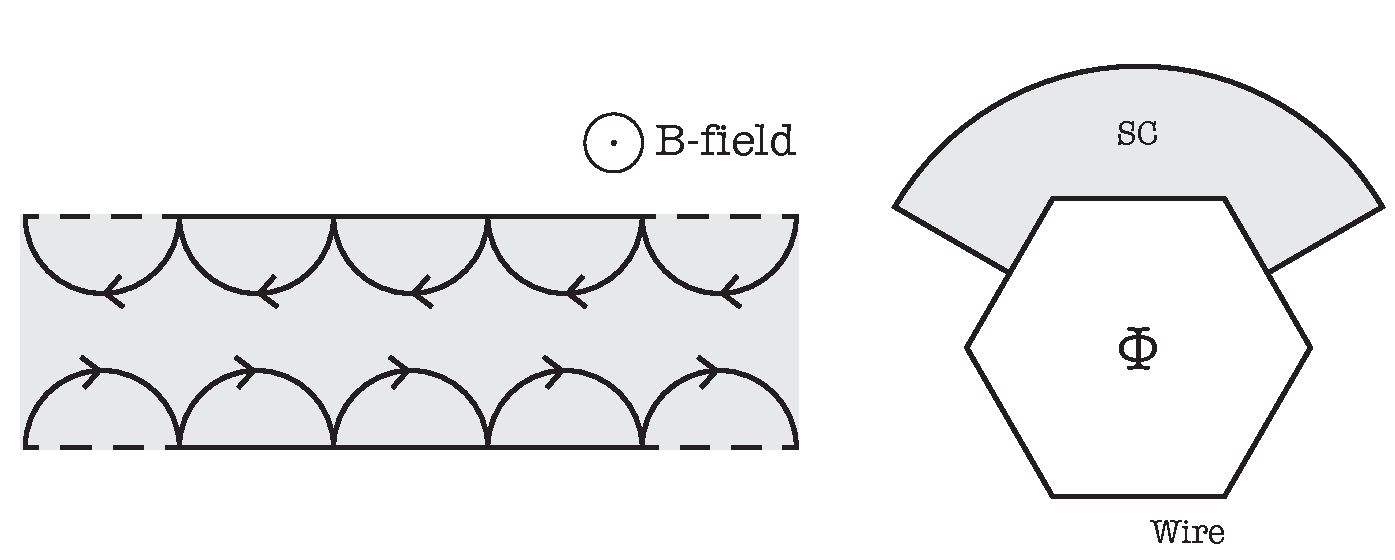
\includegraphics[width=0.95\textwidth]{chapter_introduction/figures/wires.pdf}
\par\end{centering}
\caption{Orbital effect of magnetic field influences the state of particles for both a field parallel and perpendicular to the wire axis.
A perpendicular field induces a skipping orbit motion of the electrons (left).
A magnetic field parallel to the wire shifts the energies due to the effect of magnetic flux $\Phi$.
\label{fig:wire}}
\end{figure}

We systematically study the influence of the orbital effect of the magnetic field on the symmetries of the Hamiltonian and the topological phase diagram for a 3D nanowire, whose specifics are explained in chapter \ref{sec:Model}.
Orbital effect of a magnetic field perpendicular to the wire induces skipping orbit motion of the electrons (see Fig.~\ref{fig:wire}).
The cyclotron radius \footnote{$r_{\textrm{cyclo}}=\frac{mv_{\textrm{F}}}{\textrm{e}B}$, where the Fermi velocity $v_{\textrm{F}}=\sqrt{\frac{2\mu}{m}}$.} becomes comparable to the typical wire diameters $d\sim\SI{100}{nm}$ already at the field of $\SI{0.3}{T}$, and at chemical potential corresponding to the most stable Majoranas.
In addition, a field parallel to the wire shifts the energies of each band due to the effect of magnetic flux.
We expect the shift of the energies to be comparable to the level spacing when the flux through the wire is of an order of a flux quantum.
Our findings are very different from those of Refs.~\cite{Osca2015a,Lim2012,SooLim2013} because we do not limit our analysis to a Hamiltonian with an artificially high spatial symmetry, or low dimensionality.

The theoretical background needed to understand this thesis is introduced in chapter \ref{sec:superconductivity}-\ref{sec:MBS}.
We start with superconductivity and the mean-field approximation that leads to a single particle Hamiltonian that forms the basis of our model.
This Hamiltonian has certain symmetries: this will be the topic of chapter \ref{sec:topology}.
Chapter \ref{sec:braiding} will explain the concept of braiding and will make use of the Majorana properties introduced in the previous chapter.
In chapter \ref{sec:MBS} we proceed to apply this newly learned knowledge to construct a Hamiltonian for a system that can host Majoranas.

\section{\label{sec:superconductivity}Superconductivity}

Superconductivity is a phenomenon that occurs in certain materials when cooled below a characteristic critical temperature $T_{\mathrm{C}}$.
Upon reaching this temperature, the material undergoes a phase transition that results in exactly zero electrical resistance and the expulsion of magnetic fields.
Since the discovery of superconductivity by Heike Kamerlingh Onnes in 1911, considerable efforts have been devoted to finding out how and why it works.
A good understanding of ``conventional'' superconductivity was reached by a pair of remarkable and important theories: the phenomenological Ginzburg-Landau theory and the microscopic BCS theory.
Today research is focused on: exotic superconductors, high $T_{\mathrm{C}}$ superconductors, and hybrid structures consisting of a superconductor and another material.
In this thesis, we study such hybrid structures.

\subsection{BCS theory\label{sec:BCS-theory}}

BCS theory describes superconductivity as a microscopic effect and assumes that two electrons can effectively attract due to electron-phonon coupling and form a Cooper pair.
It postulates that superconductivity is caused by a condensation of Cooper pairs at the Fermi energy\footnote{We assume zero temperature $\left(T=0\right)$, so $E_{\textrm{F}}=\mu$, where $\mu$ is the chemical potential.} $E_{\textrm{F}}$ into a boson-like state, a Bose Einstein condensate.
The model Hamiltonian in the language of second quantization equals~\cite{Gennes1999}

\begin{equation}
\mathcal{H}_{\textrm{BCS}}=\sum_{\bm{k}\sigma}\epsilon_{\bm{k}}c_{\bm{k}\sigma}^{\dagger}c_{\bm{k}\sigma}+\sum_{\bm{k}\bm{l}}V_{\bm{k}\bm{l}}c_{\bm{k}\uparrow}^{\dagger}c_{-\bm{k}\downarrow}^{\dagger}c_{-\bm{l}\downarrow}c_{\bm{l}\uparrow},\label{eq:BCS}
\end{equation}

where

\begin{tabular}{ll}
 $c$  & annihilation operator electron \tabularnewline
 $c^{\dagger}$ & creation operator electron\tabularnewline
 $\epsilon_{k}$  &  $E_{k}-\mu$\tabularnewline
$\mu$ & chemical potential\tabularnewline
$E_{k}$ & kinetic energy ($\frac{\hbar^{2}k^{2}}{2m}$)\tabularnewline
$m$ & mass\tabularnewline
 $k$  & momentum\tabularnewline
 $\sigma,\uparrow,\downarrow$  & spin of electron\tabularnewline
 $V_{\bm{kl}}$ & interaction potential.\tabularnewline
\end{tabular}


The interaction term includes only the Cooper pairs, which consist of two electrons with opposite spin (s-wave symmetry) and opposite momentum and can be denoted as $(\bm{\bm{k}}\uparrow,-\bm{k}\uparrow)$.
Finding the ground state of this so-called pairing Hamiltonian is impossible; therefore, we have to make an approximation.
A classic approximation scheme that describes the behavior of conventional superconductors remarkably well is the mean-field approximation.
First we define the quantity
\[
b_{\bm{k}}=\left\langle c_{\bm{k}\uparrow}c_{-\bm{k}\downarrow}\right\rangle ,
\]
which we use to define the so-called gap energy
\[
\Delta_{\bm{k}}=-\sum_{\bm{k'}}V_{\bm{kk'}}b_{\bm{k'}}.
\]
We write $c_{\bm{k}\uparrow}^{\dagger}c_{-\bm{k}\downarrow}^{\dagger}c_{-\bm{l}\downarrow}c_{\bm{l}\uparrow}$ from Eq.~\ref{eq:BCS} as

\begin{equation}
c_{\bm{k}\uparrow}^{\dagger}c_{-\bm{k}\downarrow}^{\dagger}c_{-\bm{l}\downarrow}c_{\bm{l}\uparrow}=\left(c_{\bm{k}\uparrow}^{\dagger}c_{-\bm{k}\downarrow}^{\dagger}-b_{\bm{k}}^{\dagger}+b_{\bm{k}}^{\dagger}\right)\left(c_{-\bm{l}\downarrow}c_{\bm{l}\uparrow}-b_{\bm{l}}+b_{\bm{l}}\right),\label{eq:MF}
\end{equation}
and expand the products.
Neglecting the second-order fluctuation term
\begin{equation}
\left(c_{\bm{k}\uparrow}^{\dagger}c_{-\bm{k}\downarrow}^{\dagger}-b_{\bm{k}}^{\dagger}\right)\left(c_{-\bm{l}\downarrow}c_{\bm{l}\uparrow}-b_{\bm{k}}\right)
\end{equation}
in Eq.~\ref{eq:MF} and using it to rewrite Eq.~\ref{eq:BCS} gives
\begin{equation}
\mathcal{H}_{\textrm{BCS}_{\textrm{MF}}}=\underset{\bm{k},\sigma}{\sum}\epsilon_{\bm{k}}c_{\bm{k}\sigma}^{\dagger}c_{\bm{k}\sigma}-\underset{\bm{k}}{\sum}\left(\Delta_{\bm{k}}c_{\bm{k}\uparrow}^{\dagger}c_{-\bm{k}\downarrow}^{\dagger}+\Delta_{\bm{k}}^{*}c_{-\bm{k}\downarrow}c_{\bm{k}\uparrow}-\Delta_{\bm{k}}b_{\bm{k}}^{*}\right),\label{eq:BCS_MF}
\end{equation}
where the last term is just a constant that can be neglected.
We now introduce Nambu spinors
\begin{equation}
\Psi_{\bm{k}}=\left(\begin{array}{c}
c_{\bm{k}\uparrow}\\
c_{-\bm{k}\downarrow}^{\dagger}
\end{array}\right)\label{eq:Nambu}
\end{equation}
and write Eq.~\ref{eq:BCS_MF} in matrix representation
\[
\mathcal{H}_{\textrm{BCS}_{\textrm{MF}}}=\underset{\bm{k}}{\sum}\Psi_{\bm{k}}^{\dagger}\underset{H_{\textrm{BdG}}}{\underbrace{\left(\begin{array}{cc}
\epsilon_{\bm{k}} & \Delta\\
\Delta_{\bm{k}}^{*} & -\epsilon_{\bm{k}}
\end{array}\right)}}\Psi_{\bm{k}}.
\]
We can diagonalize the Bogoliubov-de Gennes Hamiltonian $H_{\textrm{BdG}}$ using the unitary Boguliubov transformation matrix $U_{\textrm{B}}$ and solve the eigenvalue problem.
Alternatively, we can square $H_{\textrm{BdG}}$ which gives a diagonal matrix
\[
H_{\textrm{BdG}}^{2}=\left(\begin{array}{cc}
\epsilon_{\bm{k}}^{2}+\left|\Delta\right|^{2} & 0\\
0 & \epsilon_{\bm{k}}^{2}+\left|\Delta\right|^{2}
\end{array}\right)
\]
where we can use that the eigenvalues are the square root of the eigenvalues of $H_{\textrm{BdG}}$.
This immediately result in the spectrum
\begin{equation}
E=\pm\sqrt{\epsilon_{\bm{k}}^{2}+\left|\Delta\right|^{2}}.\label{eq:SC_spectrum}
\end{equation}

The Bogoliubov-de Gennes Hamiltonian acts on the Nambu spinors (Eq.~\ref{eq:Nambu}) whose first half is composed out of annihilation operators of electrons, and the second half out of creations operators of the same electrons.
In order to go to first quantization, we can see the latter creation operators as annihilation operators of an extra set of holes and thereby double the number of degrees of freedom in the system.

Besides the Pauli matrices that act on spin ($\sigma_{i}$ where $i\in x,y,z$) we introduce $\tau_{i}$ to act on the electron-hole degree of freedom.
The Hamiltonian becomes a $4\times4$ matrix\footnote{Here $\otimes$ denotes the Kronecker product and we usually omit $\sigma_{0}$ and $\tau_{0}$.}
\[
H_{\textrm{BdG}}=\epsilon_{k}\tau_{z}\otimes\sigma_{0}+\Delta\tau_{x}\otimes\sigma_{0}=\left(\begin{array}{cccc}
\epsilon_{k} & 0 & \Delta & 0\\
0 & \epsilon_{k} & 0 & \Delta\\
\Delta & 0 & -\epsilon_{k} & 0\\
0 & \Delta & 0 & -\epsilon_{k}
\end{array}\right)
\]
which acts on the wavefunction
\begin{equation}
\Psi=\left(\psi_{\textrm{e}\uparrow},\psi_{\textrm{e}\downarrow},\psi_{\textrm{h}\downarrow},-\psi_{\textrm{h}\uparrow}\right)^{T},\label{eq:4wf}
\end{equation}
where $\psi_{\textrm{e}}$, $\psi_{\textrm{h}}$ are the electron and hole components of the wave function, and $\psi_{\uparrow}$, $\psi_{\downarrow}$ are the spin-up and spin-down states.
Now $H_{\textrm{BdG}}$ has an additional symmetry because the holes are related to the electrons.
Symmetry will be the topic of the next chapter.


\section{\label{sec:topology}Topology and symmetry}

The concept of symmetry plays a fundamental part in physics.
For a physical system it is a very important characteristic that in many cases has a decisive effect on the behavior of the system.
For example, Noether's theorem states that each continuous symmetry of a physical system implies that a certain physical property of that system is conserved.
In condensed matter systems only three discrete symmetries are important: time-reversal symmetry $\mathcal{T}$, particle-hole symmetry $\mathcal{P}$, and chiral symmetry $\mathcal{C}$.
Wigner's theorem states that a symmetry must either be a unitary or an anti-unitary operator.
Both $\mathcal{T}$ and $\mathcal{P}$ have anti-unitary operators and may square either to $+1$ or $-1$ depending on the specifics of the system.
Chiral symmetries have a unitary operator and always squares to $+1$.
Together these three symmetries form ten symmetry classes~\cite{Altland1997}, each class characterized by the type and absence or presence of these symmetries.

Topology studies whether objects can be continuously transformed into each other.
The object that is studied in condensed matter is the Hamiltonian of a system.
If two Hamiltonians can be continuously transformed\footnote{An example of a continuous transformation from $H_{1}$ to $H_{2}$: $H=\alpha H_{1}+(1-\alpha)H_{2}$ where $\alpha=0\rightarrow1$.} into each other without changing the topological invariant: the systems are said to be topologically equivalent.
The dimensionality and symmetry class determine the type of topological invariant of a system.
For example, such a topological invariant of the system we study in this thesis indicates the presence or absence of Majoranas.

\subsection{Particle-hole symmetry\label{sec:phs}}

Mathematically a particle-hole symmetry $\mathcal{P}$ is expressed as an operator that is anti-unitary and anti-commutes with the Hamiltonian.
An example of where this symmetry manifests, is the Bogoliubov-de Gennes Hamiltonian $H_{\textrm{BdG}}$ introduced in section \ref{sec:BCS-theory}.
Here, $H_{\textrm{BdG}}$ acts on a two-component wave function $\psi_{\textrm{BdG}}=\left(u,v\right)^{T}$ with $u$ electron component and $v$ the hole component.
The symmetry of this Hamiltonian is most obvious from its dispersion relation, where each eigenstate $\psi_{E}=\left(u_{0},v_{0}\right)^{T}$ has a particle-hole symmetric partner at $\psi_{-E}=\left(\mathcal{P}u_{0},\mathcal{P}v_{0}\right)^{T}$.
In constructing $H_{\textrm{BdG}}$, we artificially doubled the degrees of freedom by considering electrons and holes separately.
Therefore, the creation operator $c^{\dagger}$ of the quasiparticle in the $\psi_{E}$ state is equal to the annihilation operator $c$ of the quasiparticle in the $\psi_{-E}$ state.
It is then clear that $\psi_{E}$ and $\psi_{-E}$ correspond to the same quasiparticle, and the creation of a quasiparticle with positive energy is identical to the annihilation of a quasiparticle with negative energy.

At zero energy, something curious happens: here we have a state $\psi_{0}$ that upon applying $\mathcal{P}$ is transformed into itself $\mathcal{P}\psi_{0}=\psi_{0}$.
This state has a creation operator $\gamma^{\dagger}$ that is identical to the annihilation operator $\gamma$ of itself, so $\gamma^{\dagger}=\gamma$.
We call this property the Majorana condition, and operators that satisfy this property are called Majorana fermions.
If we use the Majorana condition in the fermionic commutation relation
\[
\gamma^{\dagger}\gamma+\gamma\gamma^{\dagger}=1
\]
we get $\gamma^{\dagger}\gamma=1/2$ and see that the Majorana state is always half occupied.
Removing a Majorana from zero energy is, therefore, only possible if it is paired with another Majorana to form a fermionic mode, but more about Majoranas in chapter \ref{sec:braiding}.

In a one or higher dimensional system, the operator $\mathcal{P}$ will not only send $E\rightarrow-E$ but will also send the momentum $k\rightarrow-k$ as
\[
\mathcal{P^{\dagger}}H\left(k\right)\mathcal{P}=-H\left(-k\right),
\]
because $\mathcal{P}$ is an anti-unitary operator.

\subsection{Chiral symmetry\label{sec:Chiral-symmetry}}

A chiral symmetry $\mathcal{C}$ is expressed as an operator that is unitary and anti-commutes with the Hamiltonian.
A system where the lattice has two sublattices, such as the hexagonal lattice of graphene, can have a chiral symmetry if we only consider the first neighbor hopping.
If we split all the degrees of freedom into two groups (say group A and group B) the Hamiltonian can be written as
\[
H=\begin{pmatrix}0 & H_{AB}\\
H_{AB}^{\dagger} & 0
\end{pmatrix}.
\]
Here the unitary Pauli matrix $\sigma_{z}$ anti-commutes with the Hamiltonian and, therefore, is a chiral symmetry.
We can apply this chiral symmetry to the Hamiltonian as
\[
\sigma_{z}H\sigma_{z}=-H,
\]
and see that this operation makes the spectrum symmetric with respect to zero energy.
Unlike particle-hole symmetry, $\mathcal{C}$ will leave momentum untouched as
\[
\mathcal{C^{\dagger}}H\left(k\right)\mathcal{C}=-H\left(k\right),
\]
because of its unitarity property.

\subsection{Topology}

As mentioned in the introduction, the dimensionality and symmetry class determine the type of topological invariant of a system.
In this thesis, we study a system that is fundamentally of symmetry class $\mathcal{D}$; this is because the Hamiltonian has a particle-hole symmetry that squares to $+1$.  % XXX: NOT TRUE
The zero-dimensional topological invariant of symmetry class D is the sign of the Pfaffian of the Hamiltonian: $\sgn\Pf\left(H\right)$, which can only assume two values, $+1$ or $-1$.
The Pfaffian for an anti-symmetric matrix is related to the determinant as $\Pf(A)^{2}=\det(A)$.
However, in many cases, the Hamiltonian is not anti-symmetric; fortunately, we can always perform a basis transformation on a particle-hole symmetric Hamiltonian that makes it so.

We still did not mention the physical reason for why a topological invariant would change.
The topological invariant is only defined for a system with an energy gap, which means the Hamiltonian of the system has no eigenvalues in a finite interval around zero energy.
If we can continuously transform a Hamiltonian $H_{1}$ into another Hamiltonian $H_{2}$ without ever closing the energy gap, we say $H_{1}$ and $H_{2}$ are topologically equivalent, and thus have the same topological invariant.


\section{\label{sec:braiding}Braiding}

For many researchers that work on Majoranas, the ultimate motivation to study them is the fact that they have a fascinating property, non-Abelian quantum statistics.
Quantum statistic studies what happens to wavefunctions describing identical particles when their positions are exchanged in space.
In our quantum mechanics courses, we learned that particles are divided into two classes according to quantum statistics: bosons which stay the same under the exchange and fermions for which the wavefunction changes sign.
However, Majorana bound states do not belong to either of these.
The operation of exchanging two Majoranas can send the system into a different state with the same particle configuration.
Explaining how one could experimentally perform a braiding operation is beyond the scope of this thesis; therefore, we will focus on the mathematical operations that describe the braiding process.

Exchanging two Majoranas in 1D is ill-defined because it is impossible to swap them without having them collide, which would annihilate them.
We can construct a network of nanowires to form T-junctions (see Fig.~\ref{fig:Majorana-T-junction}), which allows us to exchange positions of Majoranas.
Here, one can temporarily move a Majorana to one of the unoccupied wires and perform the exchange without the Majoranas ever becoming too close to each other.

\begin{figure}
\begin{centering}
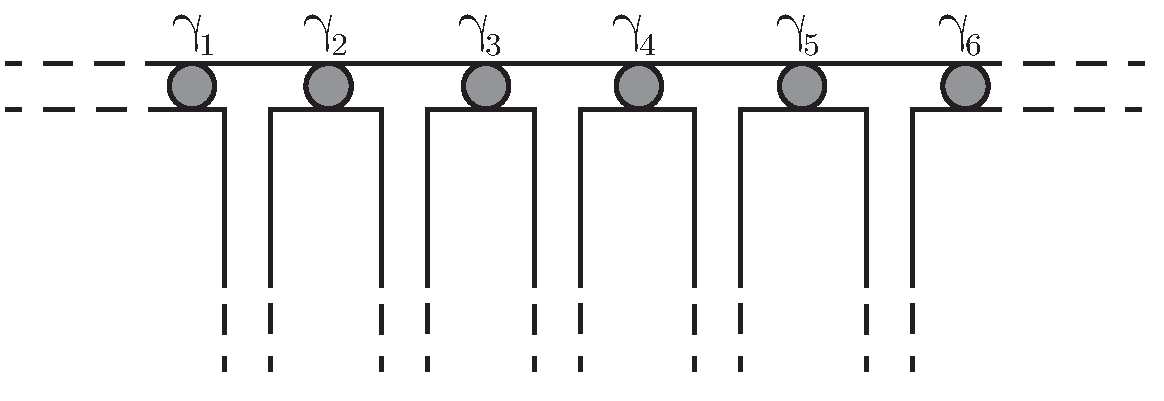
\includegraphics[width=0.95\textwidth]{chapter_introduction/figures/T-junction-network.pdf}
\par\end{centering}
\centering{}
\caption{Majorana T-junction.
The circles represent the Majoranas $\gamma_{1}...\gamma_{6}$.
This network of nanowires allows for the exchange of two Majoranas without having them collide.
This is possible by temporarily bringing a Majorana to one of the
vertical wires and then swapping the position of the other Majorana.
\label{fig:Majorana-T-junction}}
\end{figure}

The only thing that distinguishes Majoranas is their position in the network.
That means that if we exchanged two Majoranas in space, the system would look exactly the same as it looked before the exchange.
We now assume the energy spectrum is gapped for $0<E<\Delta$ with the Majorana ground state at $E=0$.
If this ground state contains several Majoranas, there will be several states all at zero energy, forming a \textquotedblleft ground state manifold\textquotedblright .
From now on we only consider the states corresponding to the Majoranas and neglect the states that live in the bulk ( $E\geq\Delta$).\\ As mentioned in chapter \ref{sec:phs}, a Majorana has only half a degree of freedom and thus, they can only be assigned quantum states in pairs.
In Fig.~\ref{fig:Majorana-T-junction} we see six Majoranas (3 pairs), but for generality lets consider $N$ pairs.
By pairing two Majoranas (two times half a degree of freedom), we can form fermionic modes that will give us two possible degenerate quantum states, either unoccupied $\ket0$ or occupied $\ket1$.
By pairing up neighboring Majoranas\foreignlanguage{english}{ $\gamma_{2n-1}$} and \foreignlanguage{english}{$\gamma_{2n}$} we get a creation operator that is its own complex conjugate $c_{n}^{\dagger}=\tfrac{1}{2}(\gamma_{2n-1}+i\gamma_{2n})$, where $c$ is a fermionic creation operator.
Each pair gives two possible quantum states, so $N$ pairs will have $2^{N}$ possible states.
We can represent every such state with a ket
\[
\left|s_{1},s_{2},\dots,s_{N}\right\rangle ,
\]
where $s_{n}$ is either unoccupied $0$ or occupied $1$.
These states form a complete basis of the Hilbert space of the set of Majoranas.

We define the fermion parity operator
\[
P_{n}\equiv1-2c_{n}^{\dagger}c_{n}=i\gamma_{2n-1}\gamma_{2n},
\]
that acts on the states and where we recognize the $c_{n}^{\dagger}c_{n}$ term as the number operator.
All basis states in the Hilbert space of Majoranas are eigenstates of $P_{n}$.
For example, we have
\[
P_{1}\left|0,\dots\right\rangle \ =(1-2c_{1}^{\dagger}c_{1})\left|0,\dots\right\rangle =+\left|0,\dots\right\rangle ,
\]

\[
P_{1}\left|1,\dots\right\rangle \ =(1-2c_{1}^{\dagger}c_{1})\left|1,\dots\right\rangle =-\left|1,\dots\right\rangle .
\]

Another essential property of Majoranas is that a pair of Majorana operators all anti-commute with each other.
So
\[
(\gamma_{1}\gamma_{2})(\gamma_{3}\gamma_{4})=(\gamma_{3}\gamma_{4})(\gamma_{1}\gamma_{2}),
\]
but when the pairs share a Majorana they do not commute anymore
\[
(\gamma_{1}\gamma_{2})(\gamma_{2}\gamma_{3})=-(\gamma_{2}\gamma_{3})(\gamma_{1}\gamma_{2}).
\]

In chapter \ref{sec:superconductivity} you might have noticed that the total particle number in the Hamiltonian is not conserved; however, the parity is conserved.
The total parity can be obtained by multiplying all parity operators
\[
P_{\textrm{tot}}=P_{1}\cdot P_{2}\cdot\,\dots\,\cdot P_{N}=i^{N}\gamma_{1}\gamma_{2}\dots\gamma_{2N}.
\]
where $P_{\textrm{tot}}$ has eigenvalues $\pm1$.
The parity is an observable and can, therefore, be experimentally measured.


We can now start to think about what would happen when we exchange two Majoranas~\cite{Ivanov2001}.
Our ground state manifold $\ket\Psi$ will never leave the ground state if we perform the exchange slowly enough.
The exchange of two Majoranas $\gamma_{n}$ and $\gamma_{m}$ will change the ground state $\left|\Psi\right\rangle \to U\left|\Psi\right\rangle $ where $U$ is a unitary operator.
The exact form of $U$ can be derived without a direct calculation.
We do this by assuming that $U$ only depends on the Majoranas involved in the exchange ( $\gamma_{n}$ and $\gamma_{m}$) and by using that the slow exchange does not change the parity of the system because the system stays gapped at all times.
Since the parity is conserved we know: $U$ commutes with the total fermion parity $[U,P_{\textrm{tot}}]=0$, and that $U$ can only depend on the product $i\gamma_{n}\gamma_{m}$.
This product is Hermitian, so we can create a unitary operator by taking the exponential of $i$ times this Hermitian operator as
\[
U\equiv\exp(\beta\gamma_{n}\gamma_{m})=\cos(\beta)+\gamma_{n}\gamma_{m}\sin(\beta),
\]
where $\beta$ is a real coefficient to be determined.
In the last equality we used $(\gamma_{n}\gamma_{m})^{2}=\gamma_{n}\gamma_{m}\gamma_{n}\gamma_{m}=-\gamma_{n}\underset{=1}{\underbrace{\gamma_{m}\gamma_{m}}}\gamma_{n}=-1$
in the Taylor expansion.


We now move to the Heisenberg picture where we look at the evolution of the Majorana operators in time
\[
\gamma_{n}\to U\gamma_{n}U^{\dagger}=\left(\cos\beta+\gamma_{n}\gamma_{m}\sin\beta\right)\gamma_{n}\left(\cos\beta+\gamma_{m}^{\dagger}\gamma_{n}^{\dagger}\sin\beta\right)
\]

\[
=\gamma_{n}\cos^{2}\beta+\left(\gamma_{n}\gamma_{m}^{\dagger}\gamma_{n}^{\dagger}+\gamma_{n}\gamma_{m}\gamma_{n}\right)\sin\beta\cos\beta+\gamma_{n}\gamma_{m}\gamma_{n}\gamma_{m}^{\dagger}\gamma_{n}^{\dagger}\sin^{2}\beta
\]

\[
=\gamma_{n}\cos^{2}\beta-\gamma_{n}^{\dagger}\sin^{2}\beta-2\gamma_{m}\sin\beta\cos\beta
\]

\[
=\gamma_{n}\cos2\beta-\gamma_{m}\sin2\beta
\]
Similarly we get
\[
\gamma_{m}\to U\gamma_{m}U^{\dagger}=\gamma_{m}\cos2\beta+\gamma_{n}\sin2\beta.
\]
After the exchange happened we know that $\gamma_{m}\to\gamma_{n}$ and $\gamma_{n}\to\gamma_{m}$, this leads to $\beta=\pm\pi/4$.
The two signs make sense; this distinguishes the clockwise and the counterclockwise exchange of the Majoranas.
We now found an operator that exchanges two Majoranas
\begin{equation}
U=\exp\left(\pm\frac{\pi}{4}\gamma_{n}\gamma_{m}\right)=\tfrac{1}{\sqrt{2}}\left(1\pm\gamma_{n}\gamma_{m}\right).\label{eq:U_nm}
\end{equation}

As an example, lets now look at what happens when we have just four Majoranas $\gamma_{1}$, $\gamma_{2}$, $\gamma_{3}$ and $\gamma_{4}$.
The four basis states in the ground state manifold are
\begin{equation}
\left|00\right\rangle ,\left|01\right\rangle ,\left|10\right\rangle ,\left|11\right\rangle ,\label{eq:basis}
\end{equation}
where the first number is the occupation number of the fermionic mode $c_{1}^{\dagger}=\tfrac{1}{2}(\gamma_{1}+i\gamma_{2})$ and the second number the occupation number of $c_{2}^{\dagger}=\tfrac{1}{2}(\gamma_{3}+i\gamma_{4})$.
For instance, if we start from the state $\left|00\right\rangle $ and we exchange $\gamma_{2}$ and $\gamma_{3}$ by applying $U_{23}=\tfrac{1}{\sqrt{2}}\left(1\pm\gamma_{2}\gamma_{3}\right)$, we obtain\footnote{See appendix \ref{chap:U_der} for derivations of $U_{nm}$.}
\[
\left|00\right\rangle \to U_{23}\left|00\right\rangle =\tfrac{1}{\sqrt{2}}\left(\left|00\right\rangle +i\left|11\right\rangle \right).
\]
Here we see a superposition of states, which is not like bosons or fermions at all, where the exchange can only change the sign.
This property makes Majoranas non-Abelian anyons, and the exchange of two non-Abelian anyons is usually called braiding.



\section{\label{sec:MBS}Creating Majoranas in a nanowire}

The combined effect of superconductivity, spin-orbit coupling, and a Zeeman field can lead to the appearance of Majoranas near the edges of the wire~\cite{Lutchyn2010,Oreg2010}.
Before we can understand why this might happen, we will study the effects of the various terms in the Hamiltonian.
The appearance of Majoranas is a topological effect and is accompanied by the change of the topological invariant $Q$ of symmetry class D.
As discussed in chapter \ref{sec:topology}, this invariant can only assume $Q=+1$ (no Majoranas) and $Q=-1$ (Majoranas present) and changes when the bandgap is closed.


\begin{figure}
\begin{centering}
\includegraphics[width=0.95\textwidth]{chapter_introduction/figures/triv_topo_bandstructure.pdf}
\par\end{centering}
\caption{Band structures of Hamiltonians with chemical potential $\mu=-0.3$
and superconducting gap $\Delta=0$ (left); $\mu=0.3$ and $\Delta=0$
(middle); $\mu=0.3$, $\Delta=0.1$.
\label{fig:triv_topo_bandstructure}}
\end{figure}

The complete model Hamiltonian is rather complicated; we will, therefore, start with a one-dimensional single band Hamiltonian in its simplest form and study the band structures while adding terms needed to make a topological band structure and ``engineer'' our way towards Majoranas.
The Hamiltonian in its simplest form is quadratic in momentum and has an off-set in chemical potential $\mu$  \begin{equation}
H=\left(\frac{\bm{p}^{2}}{2m}-\mu\right)\tau_{z},\label{eq:simple_ham}
\end{equation}
where $\tau_{z}$ is a Pauli matrix that acts on the electron-hole substructure.
The band structure for this Hamiltonian with $\mu=-0.3$ is shown in Fig.~\ref{fig:triv_topo_bandstructure} (left).
We now assume that this band structure is topologically trivial and has $Q=+1$.
The wavefunction where we doubled the degrees of freedom has four components (Eq.~\ref{eq:4wf}).
Therefore, the bands in Fig.~\ref{fig:triv_topo_bandstructure} (left) are doubly degenerate because both spin up and down is on the same energy.
The $\tau_{z}$ in the Hamiltonian ensures that the electrons are at positive energy $E$ and the holes on $-E$.


The next step is to create a bandgap closure in order to change $Q$.
This is done by raising $\mu$, which shifts the bands, see Fig.~\ref{fig:triv_topo_bandstructure} (middle).
In chapter \ref{sec:topology}, we explained that the topological invariant is only defined for a system with an energy gap.
This band structure has no bandgap, so it cannot be topological.
Further, in chapter \ref{sec:superconductivity} we saw that having a superconductor leads to a gapped spectrum (Eq.~\ref{eq:SC_spectrum}), so adding $\Delta\tau_{x}$ (which results in the the Bogoliubov-de Gennes Hamiltonian)
\[
H_{\textrm{BdG}}=\left(\frac{\bm{p}^{2}}{2m}-\mu\right)\tau_{z}+\Delta\tau_{x},
\]
creates a gap because $\tau_{x}$ mixes the electron and holes (see Fig.~\ref{fig:triv_topo_bandstructure} (right)).
We can now argue that Fig.~\ref{fig:triv_topo_bandstructure} (right) is a topological band structure because the bandgap closed and consequently: $Q$ changed.
However, $Q$ changed twice, because the doubly degenerate spin bands both crossed zero energy simultaneously, and therefore we need some more terms to reach our goal.

\subsection{Zeeman splitting}

We are now left in a state where for every eigenstate, there is at least one more eigenstate with the same energy, this is called Kramer's degeneracy, and it needs to be broken in order to make Majoranas.
\footnote{With Kramer's degeneracy, we would make two Majoranas per edge.}
To couple to spin we introduce the Zeeman field in the Hamiltonian, which now becomes
\begin{equation}
H_{\textrm{BdG}}=\left(\frac{\bm{p}^{2}}{2m}-\mu\right)\tau_{z}+\Delta\tau_{x}+\frac{1}{2}g\mu_{\textrm{B}}B\sigma_{x},\label{eq:zeeman}
\end{equation}
where $g$ is the Landé factor, $\mu_{\textrm{B}}$ the Bohr magneton and $B$ magnetic field along $x$, parallel to the wire direction.
In Fig.~\ref{fig:zeeman} band structures are plotted for different values of magnetic field.

\begin{figure}
\begin{centering}
\includegraphics[width=0.95\textwidth]{chapter_introduction/figures/zeeman.pdf}
\par\end{centering}
\caption{Band structures of Eq.~\ref{eq:zeeman} for different values of magnetic field and $\Delta=0.1$, $\mu=0.3$.
\label{fig:zeeman}}
\end{figure}
We see that the Kramer's degeneracy is broken when we turn on the magnetic field, because there are no different states with the same energy anymore.
The bands that move towards each other have opposite spin (orthogonal states), and as we see in Fig.~\ref{fig:zeeman} (middle and left), these spins do not couple.
The problem is that Zeeman conserves spin in $x$-direction, and therefore spin is still a good quantum number.
We know that Majoranas must be spinless because they are their own complex conjugate.


\subsection{Spin-orbit coupling}

The solution to this last problem is spin-orbit coupling, which in its simplest form is Rashba: $H_{\textrm{Rashba}}=-\alpha p_{x}\sigma_{y}\tau_{z}$.
The Hamiltonian is now complete and equals
\begin{equation}
H_{\textrm{BdG}}=\left(\frac{\bm{p}^{2}}{2m}-\mu\right)\tau_{z}+\Delta\tau_{x}+\frac{1}{2}g\mu_{\textrm{B}}B\sigma_{x}-\alpha p_{x}\sigma_{y}\tau_{z}.\label{eq:rashba}
\end{equation}
Lets first see why spin-orbit by itself---because is seems to couple spin---is not sufficient to break the Kramer's degeneracy and why we needed the Zeeman term in the first place.
In Fig.~\ref{fig:SO_no_zeeman} we see that upon raising $\alpha$ the different spin bands move away in either $+k$ or $-k$ direction.
However, Kramer's degeneracy is not broken because there are two states with the same energy at $k=0$.

\begin{figure}
\centering{}\includegraphics[width=0.95\textwidth]{chapter_introduction/figures/SO_no_zeeman.pdf}
\caption{Band structures of Eq.~\ref{eq:rashba} for different values of spin-orbit coupling $\alpha$ and $B=0$, $\Delta=0.1$, $\mu=0.3$.
\label{fig:SO_no_zeeman}}
\end{figure}
If we now also turn on magnetic field we see that spin-orbit opens the gap at finite $k$ (see Fig.~\ref{fig:SO_and_zeeman}).
This system will accommodate Majoranas at $E=0$ and is called topologically nontrivial, for it has no degeneracies, a gapped spectrum, and $Q=-1$.

\begin{figure}
\centering{}\includegraphics[width=0.95\textwidth]{chapter_introduction/figures/SO_and_zeeman.pdf}
\caption{Band structures of Eq.~\ref{eq:rashba} for different values of spin-orbit coupling $\alpha$ and $B=0.3$, $\Delta=0.1$, $\mu=0.3$.
\label{fig:SO_and_zeeman}}
\end{figure}


\subsection{Wavefunctions}

With a topological band structure, we expect Majoranas to appear near
the edges of the nanowires.
We can check if this happens by calculating the wavefunctions of a finite wire and plotting the probability density of the wavefunction corresponding to the lowest energy.
In Fig.~\ref{fig:wavefunction_1d} (left), we see the probability density of the lowest energy mode (the Majorana wavefunction) is indeed localized near edges of the nanowire.
The wavefunction decays exponentially with decay length $\xi$.

\begin{figure}
\begin{centering}
\includegraphics[width=0.95\textwidth]{chapter_introduction/figures/wavefunction_1d.pdf}
\par\end{centering}
\caption{Probability density and band structure of a 1D system.
The probability density of the lowest energy wavefunction (Majorana wavefunction) of a \SI{2}{\micro\metre} long nanowire (left) and a topological band structure (right) with the same parameter values, but for an infinite system.
The Majorana length $\xi$---the decay length of the wavefunction---in
the left plot is $\xi=\SI{315}{nm}$.
\label{fig:wavefunction_1d}}
\end{figure}

In 2D the model Hamiltonian (Eq.~\ref{eq:rashba}) looks very similar
\begin{equation}
H_{\textrm{BdG}}=\left(\frac{\bm{p}^{2}}{2m}-\mu\right)\tau_{z}+\Delta\tau_{x}+\frac{1}{2}g\mu_{\textrm{B}}B\sigma_{x}+\alpha\left(p_{y}\sigma_{x}-p_{x}\sigma_{y}\right)\tau_{z},\label{eq:2D_Ham}
\end{equation}
where it now also includes the transverse part of the Rashba spin-orbit.
The probability density and band structure of a 2D system is plotted in Fig.~\ref{fig:wavefunction_2d}.

\begin{figure}
\begin{centering}
\includegraphics[width=0.95\textwidth]{chapter_introduction/figures/wavefunction_2d.pdf}
\par\end{centering}
\caption{Similar to Fig~\ref{fig:wavefunction_1d}, but for a 2D system.
\label{fig:wavefunction_2d}}
\end{figure}


\subsection{Phase diagrams}

We have seen that a topological band structure leads to Majoranas near the edges of the nanowire.
In the Hamiltonian (\ref{eq:rashba}) we see a few fundamental constants or constants that are material dependent.
However, the chemical potential $\mu$ and magnetic field $B$ can be adjusted in an experiment; asking for which values of $B$ and $\mu$ the system becomes topological is therefore a valid question.
In Fig.~\ref{fig:topo_bands} we see a phase diagram, which indicates for which value of $\left(B,\mu\right)$ the system is topological.
The color intensity indicates the size of the topological bandgap, which is a measure of the quality of the Majorana.
In chapter \ref{sec:phase-diagram} we explain how to calculate a phase diagram.

In the next chapter we will extend this model to three dimensions and add the orbital effect of the magnetic field.

\begin{figure}
\begin{centering}
\includegraphics[width=0.8\textwidth]{chapter_introduction/figures/phase_diagrams_bands.pdf}
\par\end{centering}
\caption{Topological phase diagram of a 3D system.
On the left three phase diagrams with a blue dot that indicates the value of $B,\mu$ at which the band structure to the right of it is plotted.
The color in the phase diagrams depicts the topological region and its intensity the size of the topological gap.
The bottom band structure is topological, and a small gap is visible in the plot.
\label{fig:topo_bands}}
\end{figure}


\section{Structure of this thesis}

Here, we give a brief overview of the topics explored in the following chapters.
\vspace{1mm}

\subsection{Chapter~\ref{ch:introduction}: Introduction}
Abstract here for introduction
\vspace{1mm}

\subsection{Chapter~\ref{ch:adaptive}: Title here for adaptive}
Abstract here for adaptive
\vspace{1mm}

\subsection{Chapter~\ref{ch:orbitalfield}: Orbital effect of magnetic field on the Majorana phase diagram}
Studies of Majorana bound states in semiconducting nanowires frequently neglect the orbital effect of a magnetic field.
Systematically studying its role leads us to several conclusions for designing Majoranas in this system.
Specifically, we show that for experimentally relevant parameter values the orbital effect of a magnetic field has a stronger impact on the dispersion relation than the Zeeman effect.
While Majoranas do not require the presence of only one dispersion subband, we observe that the size of the Majoranas becomes unpractically large, and the band gap unpractically small, when more than one subband is filled.
Since the orbital effect of a magnetic field breaks several symmetries of the Hamiltonian, it leads to the appearance of large regions in parameter space with no band gap whenever the magnetic field is not aligned with the wire axis.
The reflection symmetry of the Hamiltonian with respect to the plane perpendicular to the wire axis guarantees that the wire stays gapped in the topologically nontrivial region as long as the field is aligned with the wire.
\vspace{1mm}

\subsection{Chapter~\ref{ch:supercurrent}: Supercurrent Interference in Few-Mode Nanowire Josephson Junctions}
Junctions created by coupling two superconductors via a semiconductor nanowire in the presence of high magnetic fields are the basis for the potential detection, fusion and braiding of Majorana bound states.
We study NbTiN/InSb nanowire/NbTiN Josephson junctions and find that the dependence of the critical current on the magnetic field exhibits gate-tunable nodes.
This is in contrast with a well-known Fraunhofer effect, under which critical current nodes form a regular pattern with a period fixed by the junction area.
Based on a realistic numerical model we conclude that the Zeeman effect induced by the magnetic field and the spin-orbit interaction in the nanowire are insufficient to explain the observed evolution of the Josephson effect.
We find the interference between the few occupied one-dimensional modes in the nanowire to be the dominant mechanism responsible for the critical current behavior.
We also report a strong  suppression of critical currents at finite magnetic fields that should be taken into account when designing circuits based on Majorana bound states.
\vspace{1mm}

\subsection{Chapter~\ref{ch:spinorbit}: Spin-Orbit Protection of Induced Superconductivity in Majorana Nanowires}
Spin-orbit interaction (SOI) plays a key role in creating Majorana zero modes in semiconductor nanowires proximity coupled to a superconductor.
We track the evolution of the induced superconducting gap in InSb nanowires coupled to a NbTiN superconductor in a large range of magnetic field strengths and orientations.
Based on realistic simulations of our devices, we reveal SOI with a strength of 0.15--0.35 eV\AA.
Our approach identifies the direction of the spin-orbit field, which is strongly affected by the superconductor geometry and electrostatic gates.
\vspace{1mm}

\subsection{Chapter~\ref{ch:zigzag}: Title here for zigzag}
Abstract here for zigzag
\vspace{1mm}

\subsection{Chapter~\ref{ch:shortjunction}: Robustness of Majorana bound states in the short-junction limit}
We study the effects of strong coupling between a superconductor and a semiconductor nanowire on the creation of the Majorana bound states, when the quasiparticle dwell time in the normal part of the nanowire is much shorter than the inverse superconducting gap.
This ``short-junction'' limit is relevant for the recent experiments using the epitaxially grown aluminum characterized by a transparent interface with the semiconductor and a small superconducting gap.
We find that the small superconducting gap does not have a strong detrimental effect on the Majorana properties.
Specifically, both the critical magnetic field required for creating a topological phase and the size of the Majorana bound states are independent of the superconducting gap.
The critical magnetic field scales with the wire cross section, while the relative importance of the orbital and Zeeman effects of the magnetic field is controlled by the material parameters only: $g$ factor, effective electron mass, and the semiconductor-superconductor interface transparency.

\subsection{Chapter~\ref{ch:weakantilocalization}: Title here for weakantilocalization}
Abstract here for weakantilocalization
\vspace{1mm}


\references{dissertation}

\chapter{Orbital effect of magnetic field on the Majorana phase diagram}
\label{ch:orbitalfield}

%% Start the actual chapter on a new page.
\newpage
\noindent 
\section{Introduction}



\references{dissertation}
\chapter{Supercurrent interference in few-mode nanowire Josephson junctions}
\label{ch:supercurrent}

%% Start the actual chapter on a new page.
\newpage
\noindent 
\section{Introduction}

Semiconductor nanowires coupled to superconductors form a promising platform for generating and investigating Majorana bound states \cite{kitaev2001unpaired, oreg2010helical, lutchyn2010majorana,mourik2012signatures, deng2016majorana, albrecht2016exponential,chen2016phasediagram}. 
Josephson weak links based on nanowires may provide additional evidence for Majorana bound states, e.g. through the fractional Josephson effect \cite{molenkamp2016abs4pi,bocquillon2016gapless,Deacon2016josephsonradiation}. 
These weak links can also become elements of Majorana-based topological quantum circuits \cite{Hyart2013braiding, Aasen2016briading, Karzig2016braiding, plugge2016majorana}.
Previous work on semiconductor nanowire Josephson junctions demonstrated supercurrent transistors \cite{doh2005tunable}, transport through few channels \cite{goffman2017conduction}, a nonsinusoidal current-phase relationship \cite{spanton2017current}, nanowire superconducting quantum interference devices (SQUIDs) \cite{vanDam2006supercurrent, szombati2015josephson}, and gate-tunable superconducting quantum bits\cite{deLange2015hyrbidnanowire,marcus2015hyrbidnanowire}.
Recent works reported Josephson effects at high magnetic fields, sufficient to generate unpaired Majorana bound states \cite{szombati2015josephson,giazaotto2015pbinas,giazotto2016magnetically,gharavi2016nb}.

In this Letter we study the critical current as a function of the magnetic field and gate voltage in nanowire Josephson junctions tuned to the mesoscopic few-mode regime.
The junctions consist of InSb weak links and NbTiN superconductor contacts.
For magnetic fields parallel to the nanowire, we observe a strong suppression of the critical current at magnetic fields on the scale of $\SI{100}{mT}$. 
When the magnetic field exceeds $\sim \SI{100}{mT}$, the critical current exhibits aperiodic local minima (nodes). 
In contrast with supercurrent diffraction in large multimode junctions, the magnetic field nodes of the critical current are strongly tunable by the voltages on local electrostatic gates, and are not uniquely determined by the junction geometry and supercurrent density distribution. 
To understand our data, we develop a numerical model of a quasiballistic few-mode nanowire of realistic geometry.
Our model includes the intrinsic spin-orbit effect, as well as the vector-potential and Zeeman effects of the external magnetic fields. 
Based on the simulations, we conclude that quantum interference between supercurrents carried by different transverse modes is the dominant mechanism responsible for both the critical current suppression, and the gate-sensitive nodes in the critical current.

\begin{figure}[ht]
\includegraphics[width=\columnwidth]figures/{fig1}
\caption{(a) Schematic superconductor ($S$)-nanowire-$S$ Josephson junction. The cross section shows cartoon wave functions of $n=3$ transverse modes and the flux $\Phi$ penetrating the area of the nanowire. The blue arrows indicate spin-resolved modes; the black dashed arrows are same-spin scattering events within the wire. All modes are coupled at the contacts. 
The directions of $B$ and the spin-orbit effective field $B_\mathrm{SO}$ are indicated. (b) Differential resistance $\mathrm{d}V/\mathrm{d}I$ versus $B$ and $I_\mathrm{bias}$.
The current bias sweep direction is from negative to positive. Data from device 1. Inset: SEM image of a typical device similar to those studied here. $S$ labels the superconducting contacts while $B$ indicates the in-plane magnetic field for device 2.}
\label{fig:figure1}
\end{figure}

Figure \ref{fig:figure1}(a) presents a schematic of a few-mode nanowire Josephson junction.
The inset of Fig.~\ref{fig:figure1}(b) shows a device similar to those used in this study and their fabrication process is described in Ref.~\onlinecite{mourik2012signatures}.
The junction consists of an InSb nanowire with a diameter of $100 \pm \SI{10}{nm}$ with 80 nm thick dc magnetron sputtered NbTiN contacts.
The wire sits on top of an array of 50 or $\SI{200}{nm}$ wide gates isolated from the junction by a dielectric. 
We report data from devices 1 and 2 in the main text and show additional data from device 3 in the Supplemental Material, Ref. ~\onlinecite{supp}.
Device 1(2) has a contact spacing of $\sim \SI{1}{\micro \m}$($\sim \SI{625}{nm}$) and the nanowire is at an angle of $25^\circ \pm 5^\circ$($0^\circ \pm 5^\circ$) with respect to $B$. 
Device 3 has a shorter contact spacing of $\sim \SI{150}{nm}$ and shows similar behavior of gate-tunable nodes but the initial critical current decay is extended to 400 mT.
The measurements were performed in a dilution refrigerator with a base temperature of $\sim\SI{60}{mK}$. 
All bias and measurement lines connected to the device are equipped with standard $RC$ and copper powder filtering at the mixing chamber stage to ensure a low electrical noise environment. 
The voltage measurements are performed in the four-terminal geometry.

We set all the gates underneath the nanowire to positive voltages, in the few-mode transparent regime in which no quantum dots are formed between the superconducting contacts, and the normal state conductance exceeds $2e^2/h$ (see the full gate trace of the supercurrent in the Supplemental Material ~\cite{supp}).

Figure \ref{fig:figure1}(b) shows a typical example of the differential resistance $\mathrm{d}V/\mathrm{d}I$ as a function of the magnitude of the magnetic field $B$ and the current bias $I_\mathrm{bias}$ in this few-mode regime, with low resistance supercurrent regions in dark blue around zero current bias. 

Note that the data at low field are asymmetric with respect to current reversal. Only one sweep direction is plotted for the rest of the figures.

A strong decrease of the switching current is observed from $B=\SI{0}{T}$ to $B=100-\SI{200}{mT}$. 
Beyond the initial decrease, the critical current exhibits nonmonotonic behavior with multiple nodes and lobes. 
Despite the \SI{1}{\micro \meter} contact separation, the supercurrent can be resolved up to fields as high as $B=\SI{2}{T}$, which is comparable to the estimated strength of the effective spin-orbit field $B_\mathrm{SO}$.
At finite magnetic fields where the Josephson energy is suppressed the sharp switching behavior is replaced with a smooth transition to a higher resistance state. 
In voltage-biased measurements, this manifests as a zero-bias conductance peak (see Supplemental Material ~\cite{supp}). 
This signal can mimic the onset of the topological phase since it is also associated with the zero-bias conductance peak that appears at a finite magnetic field.

\begin{figure}[t]
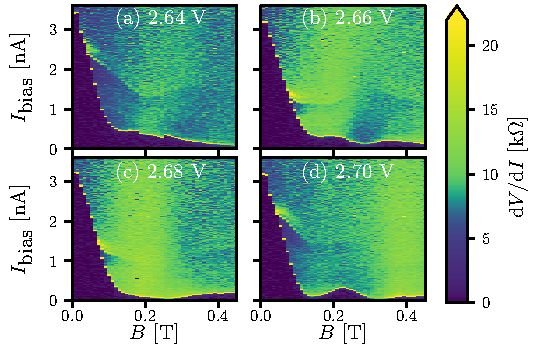
\includegraphics[width=\columnwidth]{figures/fig2.pdf}
\caption{(a)-(d) $\mathrm{d}V/\mathrm{d}I$ vs $B$ and $I_\mathrm{bias}$ for different gate voltage settings $V_\mathrm{g}$ indicated above each panel.  Data from device 2; see the Supplemental Material~\cite{supp} for the scanning electron micrograph of the device with the tuned gate marked.}
\label{fig:figure2}
\end{figure}

We now qualitatively discuss the possible explanations for the behavior observed in Fig. \ref{fig:figure1}(b).
Zeeman splitting can induce $0-\pi$-junction transitions which result in an oscillatory Josephson energy as a function of the magnetic field \cite{bulaevskii1977superconducting,  buzdin1982critical, demler1997superconducting}. 
This alternating $0-\pi$ junction behavior is due to spin-up and spin-down channels acquiring different phases as they travel across the junction [Fig. \ref{fig:figure1}(a)]. 
However, in our junctions a strong spin-orbit effective field, which has been reported to point perpendicular to the nanowire \cite{nadj2012spectroscopy}, reduces the relative phase shifts of spin-up and spin-down and lifts the nodes in the supercurrent\cite{shumeiko2008, yokoyama2014anomalous,yokoyama2014magnetic}.
For the spin-orbit strength previously reported in InSb nanowires \cite{nadj2012spectroscopy, vanweperen2015spinorbit}, we estimate an effective spin-orbit field $B_{\rm SO} \sim 1-\SI{2}{T}$ for a chemical potential value in the middle of the subband.
Therefore, we do not expect the occurrence of $0-\pi$-transitions in ballistic nanowires for fields much lower than this typical value of $B_{\rm SO}$, unless the chemical potential is close to a transverse mode edge (within $1-\SI{2}{meV}$), where $B_{\rm SO}$ is suppressed.
Given the typical mode spacing of $10-\SI{20}{meV}$~\cite{vanweperen2012quantized,kammhuber2016conductance}, in combination with the occurrence of several nodes well below \SI{1}{T}, the Zeeman $\pi$-junction effect is an unlikely explanation for all of the critical current nodes observed here for generic device settings.

Supercurrents carried by different transverse modes would also acquire different phase shifts and interfere due to mode mixing within the wire or at the contact between the nanowire and the superconductor lead~\cite{PhysRevB.91.245436}. 
Such interference is analogous to the Fraunhofer effect in wide uniform junctions: it becomes relevant when a single superconducting flux quantum is threaded through the nanowire cross section, a regime that is reached for $B \approx \SI{0.25}{T}$, well within the range of the present study. 
Comparison of the experimental and numerical data in this Letter suggests that this is the effect that dominates the magnetic field dependence of the critical current.

Transitions in and out of the topological superconducting phase in the nanowire segments covered by the superconductors were also predicted to induce reentrant critical current\cite{san2014mapping}. 
Although we used devices similar to those presented in recent Majorana experiments \cite{mourik2012signatures,Zhang2016ballisticmajoranadevice,chen2016phasediagram}, here we did not gate tune the regions of the wire underneath the superconducting contacts into the topological regime. An accidental topological regime occurring on both sides of the junction in multiple devices is an unlikely explanation for the generic observations reported here. 

Figure~\ref{fig:figure2} shows a typical sequence of magnetic field dependences of the critical current, obtained by adjusting one of the narrow local gates. 
The critical current exhibits multiple nodes [Fig.~\ref{fig:figure2}(d)], just a single node [Fig.~\ref{fig:figure2}(c)], or no node [Fig.~\ref{fig:figure2}(a)] in the same field range.
At some nodes the critical current goes to zero, while a nonzero supercurrent is observed at other nodes. 
No periodic patterns such as those characteristic of a dc-SQUID or a uniform junction are observed. 
Note that slight changes in the gate voltage are sufficient to dramatically alter the magnetic field evolution curve; the corresponding change in chemical potential $\Delta \mu$ is small ($\Delta \mu < \SI{1}{\milli \electronvolt}$) compared with the typical intermode spacing ($\sim \SI{15}{\milli \electronvolt}$). 
Furthermore, the gate used only tunes a \SI{100}{\nano \meter} segment of the \SI{650}{\nano \meter} long junction.

Typical gate sweeps of the supercurrent are presented in Fig.~\ref{fig:figure3}. 
The critical current is strongly reduced at fields above \SI{100}{\milli \tesla} irrespective of the gate voltage. 
At all fields, the supercurrent is strongly modulated by the gate voltage. 
However, gate voltages at which nodes in the critical current occur differ for each magnetic field. 
Thus, no straightforward connection can be made between the zero-field critical current and node positions at a finite field, see also Fig.~\ref{fig:figure5}(a). 

\begin{figure}
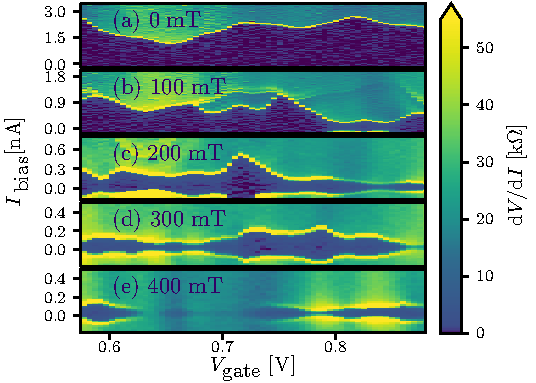
\includegraphics[width=\columnwidth]{figures/fig3.pdf}
\caption{(a)-(e) $\mathrm{d}V/\mathrm{d}I$ vs $V_\mathrm{g}$ and $I_\mathrm{bias}$ at different $B$ (indicated within each panel). Data from device 2. The gate used for tuning is different from that used in Fig.~\ref{fig:figure2}, see the Supplemental Material~\cite{supp}. }
\label{fig:figure3}
\end{figure}

\begin{figure*}[t]
\includegraphics[width=\textwidth]figures/{fig4}
\caption{Critical current and corresponding ground state phase difference for different combinations of terms in the Hamiltonian.
The Zeeman effect ($g=50$) is present in all of the curves.
Only the system corresponding to the red curve labeled with $l_\textrm{mfp}=\SI{250}{nm}$ includes disorder, for which the critical current is multiplied by a factor of 6. The simulation is performed at $T=\SI{100}{mK}$.
The curves in panels (a) and (b) are for a single spinful transverse mode ($\mu=\SI{10}{meV}$).
Panels (c) and (d) are for the multimode (three transverse or six spin-full modes) regime ($\mu=\SI{20}{meV}$).
The vertical thick dashed light blue lines in (a) and (c) indicate the positions of $0-\pi$ transitions in the absence of disorder and with $\alpha = 0$, $\bm{A}=0$.
Where not specified, the other constant simulation parameters are $\alpha=\SI{20}{\nm \meV}$, $m_\textrm{eff}=0.015 m_\textrm{e}$, $\Delta_\textrm{ind}=\SI{0.250}{meV}$; the lattice constant $a=\SI{8}{nm}$, the nanowire diameter $d_1=\SI{104}{nm}$, the outer diameter (with superconductor) $d_2=\SI{120}{nm}$, and the superconductor coverage angle (see the Supplemental Material~\cite{supp}, Fig.6) $\phi=135\si{\degree}$. For plots of corresponding current-phase relationships, Josephson energies, and numerical geometry, see the Supplemental Material ~\cite{supp}, Fig. 6-9.
}
\label{fig:critical_currents}
\end{figure*}

In order to understand the magnetic field evolution of the Josephson effect, we develop an effective low-energy model of a spin-orbit and Zeeman-coupled few-mode nanowire, covered by superconductors at both ends. 
We define $x$ as the direction along the wire, $y$ perpendicular to the wire in the plane of the substrate, and $z$ perpendicular to both wire and substrate. 
The corresponding Hamiltonian reads
\begin{align}
H = &\left(\frac{\bm{p}^2}{2m^*}-\mu + \delta U\right)\tau_z + \alpha (p_x \sigma_y - p_y \sigma_x)\tau_z \nonumber \\ &+ g \mu_B \bm{B}\cdot\boldsymbol{\sigma} + \Delta \tau_x. 
\label{eq:H}
\end{align}
Here $\bm{p}=-i\hbar\nabla+e\bm{A}\tau_z$  is the canonical momentum,  where $e$ is the electron charge, and $\bm{A}={\left[ B_y z - B_z y,\; 0,\; B_x y\right]}^{T}$ is the vector potential chosen such that it does not depend on $x$. 
Further, $m^*$ is the effective mass, $\mu$ is the chemical potential controlling the number of occupied subbands in the wire, $\alpha$ is the strength of Rashba spin-orbit interaction, $g$ is the Land{\'e} $g$-factor, $\mu_\mathrm{B}$ is the Bohr magneton, and $\Delta$ is the superconducting pairing potential.
The Pauli matrices $\sigma_i$ and $\tau_i$ act in spin and electron-hole spaces, respectively.
We assume that the electric field generated by the substrate points along the $z$ direction, such that the Rashba spin orbit acts in the $xy$\kern-.05ex-plane, which is at low energies equivalent to an effective magnetic field $\bm{B}_{\rm SO}\parallel\hat{y}$.
We include the vector potential in the tight-binding system using the Peierls substitution \cite{hofstadter_energy_1976}.
Finally, we include an uncorrelated on-site disorder $\delta U \in [-U, U]$, with $U$ the disorder strength, which we parametrize by a normal state mean free path $l_\textrm{mfp}$. \cite{beenakker1997random}$^\textrm{,}$\footnote{To determine $l_\textrm{mfp}$ we calculate a disorder-averaged normal state conductance $g$ and evaluate the mean free path $l_{mfp}$ by fitting, $g=g_0 N_\textrm{ch} / (1 + L / l_\textrm{mfp})$, with $N_\textrm{ch}$ the number of conduction channels, and $g_0$ conductance quantum.}

We perform numerical simulations of the Hamiltonian \eqref{eq:H} on a 3D lattice in a realistic nanowire Josephson junction geometry. 
The critical current is calculated using the algorithm described in Ref.~\onlinecite{ostroukh2016two} and the Kwant code \cite{groth_kwant}.
We note that for moderately damped and overdamped Josephson junctions, such as those studied here, the theoretical $I_c$ closely follows the experimentally measured switching current \cite{kautz1990noise}. 
The source code and the specific parameter values are available in the Supplemental Material ~\cite{supp}.
The full set of materials, including computed raw data and experimental data, is available in Ref.~\onlinecite{data}.

Numerical results are presented in Figs. \ref{fig:critical_currents} and \ref{fig:figure5}(b).
First, we discuss the case of only a single transverse mode occupied [Figs.~\ref{fig:critical_currents}(a) and ~\ref{fig:critical_currents}(b)], which is pedagogical but does not correspond to the experimental regime.
When all field-related terms of Eq.~\eqref{eq:H} are included ($\bm{A}\neq 0$, $\alpha \neq 0$), we observe a monotonic decay of the critical current much more gradual than in the experiment, due to the absence of the intermode interference effect in the single-mode regime.
The $\pi$-junction transitions do not appear up to fields of order $\SI{0.5}{T}$ due to the strong spin-orbit effective field, which keeps spin-up and spin-down at the same energy so that they acquire the same phase shifts traversing the junction.
The critical current eventually decays because the Zeeman term overtakes the spin-orbit term at fields greater than \SI{0.5}{\tesla}. 
When the spin-orbit term is turned off ($\alpha = 0$), we see several $0-\pi$ transitions taking place within the studied field range, confirmed by the ground state phase switching between 0 and $\pi$ at a series of magnetic fields [Fig.~\ref{fig:critical_currents}(b)].

The experimentally relevant regime is when several transverse modes are occupied. 
The measurements display three qualitative features: (i) the initial critical current at $B=\SI{0}{T}$ is strongly suppressed within $100-200$mT; (ii) the critical current then revives and continues to display nodes of variable depth and periodicity; (iii) this revival of the critical current after suppression is about 10\% of its original value at $B=\SI{0}{T}$.
Models that neglect the orbital effect display either a slow monotonic decay of the critical current (spin-orbit included, $\alpha \neq 0$), or regular critical current nodes due to $0-\pi$ transitions (no spin-orbit, $\alpha=0$) [Fig.~\ref{fig:critical_currents}(d)], as in the single-mode case.
When orbital effects are included, $\bm{A}\neq 0$, observations (i) and (ii) are reproduced but the revival of the critical current after initial suppression is still strong.
Inclusion of a realistic amount of disorder, which creates additional interference paths and suppresses supercurrent further, reproduces all observations (i), (ii), and (iii).
Thus, we conclude that the experiment is best reproduced when $\bm{A}\neq 0, \alpha \neq 0$ and weak disorder that induces intermode scattering is included within the junction model.

The inclusion of disorder in the multimode regime breaks mirror symmetry~\cite{yokoyama2014anomalous,yokoyama2014magnetic} and generates a spin-orbit field along the external magnetic field \textit{B}, which gives rise to a nonsymmetric current-phase relation, inducing a $\varphi_0$ junction (see the Supplemental Material ~\cite{supp}, Sec. VIII, for a detailed explanation). 
The ground state phase of the $\varphi_0$ junction can continuously change between 0 and $\pi$ [red trace in Fig.~\ref{fig:critical_currents}(d)]. 
Experimental verification of such phase-related effects is not possible in the two-terminal junction geometry used here, it requires phase-sensitive experiments in the SQUID geometry.

\begin{figure}[t]
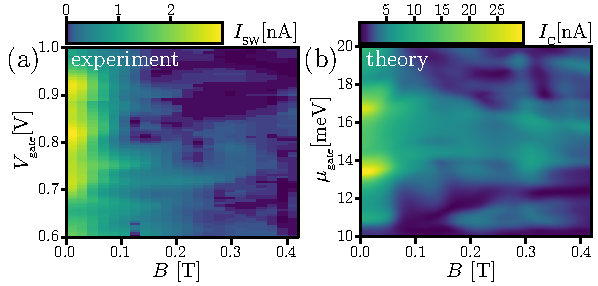
\includegraphics[width=\columnwidth]{figures/fig5.pdf}
\caption{Comparison between experimental (a) and numerical (b) results.
The parameters for the numerical simulations are the same as in Figs. \ref{fig:critical_currents}(c) and \ref{fig:critical_currents}(d), red curve.
The range of the chemical potential in the gated region ($\mu_{\textrm{gate}}$) is chosen using Ref. \onlinecite{vuik}. The experimental data are taken with device 2.}
\label{fig:figure5}
\end{figure}

In Fig.~\ref{fig:figure5} we compare side-by-side experiment and simulations via field-versus-gate maps of the supercurrent. 
In Fig.~\ref{fig:figure5}(a), the switching current from a set of $\mathrm{d}V/\mathrm{d}I$ vs. $I_\textrm{bias}$ traces similar to those in Fig.~\ref{fig:figure3} was extracted from device 2 (see the Supplemental Material ~\cite{supp} for algorithm details). 
Beyond the decay of the switching current on the scale of $\SI{100}{mT}$, the experimental data show a complex evolution of switching current maxima and minima in gate-field space. 
Characteristic features of this evolution are reproduced by our simulation shown in Fig.~\ref{fig:figure5}(b).
In particular, the experimentally observed magnetic field scale of initial supercurrent decay is reproduced in the simulation.
Furthermore, the gate-tunable maxima and minima of the critical current are recovered in our model; both in experiment and simulation these do not evolve in a regular fashion (a consequence of the complexly shaped interference trajectories). 
This qualitative agreement found additionally substantiates the applicability of our model to the experimental results.

Our results are instrumental for modeling Majorana setups. 
Specifically, the decrease of Josephson energy by an order of magnitude is observed at fields at which the onset of topological superconductivity is reported. 
This effect should, therefore, be taken into account in efforts to realize recent proposals for fusion and braiding of Majorana fermions \cite{Hyart2013braiding, Aasen2016briading, plugge2016majorana, Karzig2016braiding}, especially in those that rely on controlling the Josephson coupling \cite{Hyart2013braiding, Aasen2016briading, plugge2016majorana}. 
Our findings are applicable not only to bottom-up grown nanowires and networks but also to scalable few-mode junctions fabricated out of two-dimensional electron gases. \cite{nichelle2017scalingzbp,lee2017inas2deg} 
We suggest that in such devices narrow multimode nanowires should be used. 
At the magnetic field strengths required for braiding the many modes would facilitate strong Josephson coupling, whereas a small diameter prevents its suppression due to supercurrent interference.

Phase-sensitive measurements in the SQUID loop geometry will reveal effects  such as the Zeeman-induced  $\pi$ junction and the spin-orbit induced $\varphi_0$ junction, which our study identifies numerically but does not access experimentally. 
Single quantum mode junctions are within reach thanks to the recent demonstration of quantum point contacts in InSb nanowires at a zero magnetic field \cite{kammhuber2016conductance}. 
In that regime phenomena such as induced $p$-wave superconductivity can be studied in a unique gate-tunable setup, when tuning down to a single spin-polarized mode in the weak link. 
The results are also applicable to other interesting material systems where spin-orbit, orbital,  and Zeeman effects interplay - systems such as Ge/Si, PbS, InAs, and  Bi nanowires and carbon nanotubes. \cite{cleuziou2006carbon}

\textit{Acknowledgments.} This work has been supported by the European Research Council, the Netherlands Organization for Scientific Research (NWO), the Foundation for Fundamental Research on Matter (FOM), and Microsoft Corporation Station Q.
V.M. was supported by a Niels Stensen Fellowship for part of the research. 
A.R.A., D.I.P., and S.M.F. are grateful to KITP, where part of the research was conducted with the support of NSF Grant No. PHY11-25915. S.M.F acknowledges NSF Grant No. DMR-125296, S.M.F., L.P.K. and E.P.A.M.B. acknowledge ONR. 
D.I.P. thanks NSERC, CIFAR, and the Max Planck - UBC Centre for Quantum Materials for support.

\bibliography{bibliography.bib}


\references{dissertation}
\chapter{Spin-orbit protection of induced superconductivity in Majorana nanowires}
\label{ch:spinorbit}

%% Start the actual chapter on a new page.
\newpage
\noindent 
\section{Introduction}



\references{dissertation}
\chapter{Enhanced proximity effect in zigzag-shaped Majorana Josephson junctions}
\label{ch:zigzag}

%% Start the actual chapter on a new page.
\newpage
\noindent 
\section{Introduction}

\cite{Beenakker1992} % XXX: it needs a citation

\references{dissertation}

\chapter{Robustness of Majorana bound states in the short-junction limit}
\label{ch:shortjunction}

\blfootnote{This chapter has been previously published as
Doru Sticlet, Bas Nijholt, and Anton R. Akhmerov, \textit{Robustness of Majorana bound states in the short-junction limit}, \href{https://doi.org/10.1103/PhysRevB.95.115421}{Phys. Rev. B \textbf{95}, 115421, (2017)}
}
\blfootnote{My contributions to this work are developing and performing the numerical simulations of the three-dimensional models and writing the parts of the paper related to them.}

%% Start the actual chapter on a new page.
\newpage
\noindent

\section{Introduction}
\co{Long vs short Josephson junction}
The theory of normal conductor-superconductor (NS) hybrid systems distinguishes two limiting cases: long and short junctions.
In long junctions, the dwell time $\tau_\textrm{dw}$ of a quasiparticle inside the normal region is much larger than the time $\hbar/\Delta$ it spends inside the superconductor (with $\Delta$ the superconducting gap).
In this limit the induced gap inside the semiconductor is equal to $\hbar/\tau_{\textrm{dw}}$, and therefore it varies for different bound states.
In the short-junction or strong-coupling limit, the quasiparticles spend most of their time inside the superconductor, while the normal region effectively acts as a delta function scatterer.
Then in the presence of time-reversal symmetry, the induced gap is close to $\Delta$ for every single Andreev bound state.
In the short-junction limit Andreev bound states have the most weight in the superconductor, and therefore the conventional approach of integrating out the superconductor and obtaining an effective Hamiltonian of the normal system becomes inefficient due to the strong energy dependence of the effective Hamiltonian.

\co{MBS in short-junction limit}
Systematically studying the short-junction limit is relevant for the creation of Majorana bound states (MBS)~\cite{Qi2011, Leijnse2012, Alicea2012, Beenakker2013, Elliott2015} in semiconductor nanowires~\cite{Lutchyn2010, Oreg2010} partially coated with epitaxially grown aluminum that have high interface quality.
These systems were observed to have a well-developed hard induced gap comparable to the gap in the bare Al~\cite{Chang2015}, and subsequently showed zero bias peaks~\cite{Deng2016} and suppressed splitting of low energy states characteristic to MBS~\cite{Albrecht2016}.
The theoretical description of the response of strongly coupled zero-dimensional NS junctions to magnetic field was analyzed in Ref.~\cite{Cole2015}, where the authors report a strong suppression of the effective $g$ factor, potentially leading to the impossibility of inducing a topological phase at magnetic fields below the Clogston limit~\cite{Clogston1962}.

\co{Use scattering formalism}
Here we extend the analysis of Ref.~\cite{Cole2015} using the scattering formalism that allows us to capture the nonlinear features of the spectrum, and by considering higher-dimensional systems with translational invariance.
The scattering formalism has been routinely applied to short junctions in mesoscopic physics [for review see~\cite{Beenakker2005}].
Relevant works to the present study are on two-dimensional electronic gases with spin-orbit interactions~\cite{Bezuglyi2002, Dimitrova2006}.
However, in Majorana literature the use of the scattering formalism has been limited~\cite{Cheng2012}.
The equivalent of the scattering formalism using the effective Hamiltonian approach amounts to introducing an effective self-energy $\Sigma(E)$ which has a proper dependence on energy $E$~\cite{Liu2012, Stanescu2013, Peng2015} and then neglecting the energy term in the nonlinear eigenvalue problem $[H-\Sigma(E)]\psi = E\psi$, as done in, e.~g.,~Ref.~\cite{Poeyhoenen2016}.

\co{We find that it is not so bad}
Our overall findings are favorable for the creation of MBS in Al-based NS systems.
Specifically, we find that:
\begin{itemize}
\item The critical magnetic field $B_*$ required to induce a topological phase is independent of the superconducting gap.
 This is valid also beyond the short-junction limit, as long as penetration of magnetic field into the superconductor is negligible.
\item Since $B_*$ is inversely proportional to the wire cross section, the device design can be used to adjust $B_*$ within a broad range.
\item The localization length $\xi_M$ of the MBS does not depend on the superconducting gap, and in optimal conditions it is proportional to the spin-orbit length $l_\textrm{SO}$.
\item Finally, if the interface between the semiconductor and the superconductor has high transparency $T$, then $B_*$ becomes only a slowly varying function of the chemical potential $\mu$, as opposed to its usual oscillatory behavior on the scale of the mode spacing in the nanowire~\cite{Wimmer2010, Lutchyn2011}.
\end{itemize}
Our analytical calculations fully coincide with the results obtained using a numerical scattering approach to short junctions and exact diagonalization of a discretized tight-binding Hamiltonian.
While these conclusions are favorable for the prospect of using weak superconductors for MBS creation, we note that the effects of disorder in the superconductor are not systematically treated here.
Disorder has been recently predicted to have a strong detrimental effect on the creation of MBS in systems that are in the short-junction limit~\cite{Cole2016}.

\co{Organization of the chapter}
This chapter is organized as follows.
Section~\ref{sec:formalism} contains a pedagogical review of scattering formalism for the calculation of Andreev spectrum.
The following Sec.~\ref{sec:jjintro} presents scaling arguments supporting our conclusions.
In Sec.~\ref{sec:1stmodel} we compute the dispersion relation of a planar NS junction and discuss the typical device parameters.
Section~\ref{sec:topphases} investigates the Majorana phase diagram and the behavior of the MBS decay length.
In Sec.~\ref{sec:finite} we compare the predictions of Sec.~\ref{sec:topphases} with numerical diagonalization of finite junctions.
Section~\ref{sec:orb} estimates the orbital effect of the magnetic field by computing the Andreev spectrum in a cylindrical geometry in a thin shell limit.
In Sec.~\ref{sec:3d} we confirm our findings using a numerically computed Majorana phase diagram of a three-dimensional model.
Lastly, section~\ref{sec:conc} sums up our conclusions.

\section{Scattering matrix formalism and the short-junction limit}
\label{sec:formalism}
This section reviews the scattering approach to calculating the Andreev bound state spectrum and may be skipped by expert readers.
We start by considering a general NS junction with $n$ superconducting terminals~\cite{Heck2014}.
We use the case $n=1$ in Secs.~\ref{sec:1stmodel},~\ref{sec:topphases},~\ref{sec:3d} and $n=2$ in Sec.~\ref{sec:orb}.

\co{Andreev bound states condition.}
The levels with $|E|<\Delta$ are Andreev bound states, i.e., coherent superpositions of electron and hole excitations which occur due to Andreev reflections~\cite{Andreev1964} at the interface between the normal region and the superconducting terminals.
The wave function quantization condition on the wave function requires that the total sequence of scattering events results in a phase shift of $2\pi n$.
For the vector of modes $\psi$ incoming from the superconductor to the normal region this condition reads:
\begin{equation}\label{bound}
S_A S_N\psi=\psi.
\end{equation}
Here $S_N$ is the scattering matrix of the normal region, and $S_A$ the scattering matrix of Andreev reflection processes in the superconducting terminals.
The mode vector has electron and hole components $\psi=(\psi_e, \psi_h)$.

\co{Different bases}
The Andreev reflection matrix assumes a universal form when the superconductor has $s$-wave pairing without any sources of time-reversal symmetry breaking and additionally when the Andreev approximation holds (when the Fermi energy in the superconductor is much larger than $\Delta$).
In the literature, the Andreev spectrum is often calculated in systems where the superconductor Hamiltonian has full spin-rotation invariance (an appropriate approximation for aluminum), making the spin basis a natural choice of basis of $\psi$.
Yet the universal structure of the Andreev reflection matrix does not change in the presence of spin-orbit coupling in the superconductor.
However, in that case it is impossible to choose a spin basis due to lack of spin conservation and it is more appropriate to use a basis where the outgoing modes are time reversed of the incoming modes~\cite{Bardarson2008}.
Throughout this chapter we work in the latter basis but explain the relation to the more commonly used spin basis for reference at the end of this section.
Importantly, we neglect the time-reversal symmetry breaking perturbations in the superconductor, restricting ourselves to magnetic fields much lower than critical.

\co{Normal state scattering matrix.}
The scattering matrix of the normal region is block diagonal in the Nambu space:
\begin{equation}
S_N(E,\mathbf k)=\pmat{S_e(E,\mathbf k) & 0 \\
0 & S_h(E,\mathbf k)},
\end{equation}
where $S_e$ and $S_h$ are the scattering matrices of electrons and holes.
We consider NS junctions with a translational symmetry, and therefore the scattering matrices may depend on the wave vector $\mathbf k$ along the translationally invariant directions.
We choose the hole modes $\psi_e$ as particle-hole partners of the electron modes $\psi_e$.
In this basis the particle-hole symmetry of the scattering matrix reads:
\begin{equation}
\tau_x S^*_N(E,\mathbf k)\tau_x=S_N(-E,-\mathbf k),\label{eq:phs}
\end{equation}
Using the block-diagonal structure of $S_N$ it follows that the normal scattering matrix of holes is the conjugate of the scattering matrix for electrons, at opposite energy and momentum~\cite{Beenakker2015}:
\begin{equation}\label{phs}
S_h(E,\mathbf k)=S_e^*(-E,-\mathbf k).
\end{equation}

\co{Andreev reflection matrix}
In the same basis, the Andreev reflection matrix reads:
\begin{equation}\label{areflmat}
S_A=\alpha(E)R,\quad R=\pmat{0 & r\\ -r^* & 0},
\quad r=\oplus_j e^{i\phi_j},
\end{equation}
where the index $j$ runs over the terminals, $\phi_j$ is the superconducting phase in lead $j$, and $\alpha(E)=\exp(-i\arccos(E/\Delta))$~\cite{Beenakker1991}.

Following Ref.~\cite{Beenakker1991}, eliminating $\psi$ from Eq.~\eqref{bound}, and using an expression for a block matrix determinant one immediately arrives to a determinantal equation for the bound state energies:
\begin{equation}\label{det}
\det[
1+\alpha^2(E)r^*S_e(E,\mathbf k)rS^*_e(-E,-\mathbf k)
]=0.
\end{equation}
The short-junction limit allows us to further simplify the calculation of the Andreev bound state energies when Thouless energy $E_\textrm{Th} \equiv \hbar/\tau_\textrm{dw} \gg \Delta$.
Thouless energy is the typical energy scale for the matrix elements to change appreciably, therefore in the short-junction limit $S_N(E, \mathbf k) \approx S_N(0, \mathbf k)$ for any $E\lesssim \Delta$.
After replacing $S_e(E)$ with $S_e(0)$, the only energy-dependent term remaining in Eq.~\eqref{bound} is the coefficient $\alpha(E)$.
Since the scattering matrices are invertible, Eq.~\eqref{bound} reads:
\begin{equation}
RS_N\psi
=\alpha^{-1}(E)\psi,\textrm{ or }
S_N^{-1}R^{-1}\psi
=\alpha(E)\psi.
\end{equation}
Adding the two equations yields the following energy eigenproblem:
\begin{equation}
\frac{1}{2}[RS_N+S_N^{-1}R^{-1}]\psi
=\frac{E}{\Delta}\psi.
\end{equation}
Further squaring this equation and using the unitarity of the scattering matrices $S_A$ and $S_N$ we arrive to the eigenproblem expression for the Andreev spectrum:
\begin{equation}\label{nsspec}
\left\{
\frac{1}{2}-\frac{1}{4}
\big[
S_e^\dag(\mathbf k)rS_e^T(-\mathbf k)r^*+\mathrm{H.c.}
\big]
\right\}\psi_e=\frac{E^2}{\Delta^2}\psi_e,
\end{equation}
where the energy argument is suppressed, since $S_e$ is evaluated at $E=0$.
If there is only a single superconducting terminal, the Andreev reflection matrix $r$ reduces to a phase factor, which fully drops out from Eq.~\eqref{nsspec}, as required by gauge invariance.

If the spin is conserved, the above derivation is nearly identical in the spin basis.
The scattering matrices in the spin basis $\tilde S_e$ and $\tilde r$ are related to the basis of time-reversed modes by a transformation
\begin{equation}
\tilde S_{e}=-i\sigma_yS_{e},\quad\tilde r=-i\sigma_y\oplus_j e^{i\phi_j},
\end{equation}
with the Pauli matrices $\bm\sigma$ spin operators and $\sigma_0$ an identity matrix.
The symmetry condition~\eqref{phs}, equation~\eqref{det} for the Andreev spectrum, and eigenproblem for the spectrum in short-junction approximation~\eqref{nsspec} are identical in both bases upon replacing $S_e$ and $r$ with $\tilde S_e$ and $\tilde r$.


\section{Scaling arguments for the MBS properties in the short-junction limit}
\label{sec:jjintro}
\co{Nothing depends on the superconducting gap}
The superconducting gap enters only as an overall prefactor of the Andreev state energies in Eq.~\eqref{nsspec}, while the specific spectrum depends only on the normal state scattering matrix $S_e$.
This simplification allows us to draw most of our conclusions about MBS properties solely using universal arguments and not by solving a specific model.
For instance, since the Majorana phase transition occurs when Eq.~\eqref{nsspec} has a zero-energy solution, the critical field $B_*$ does not depend on $\Delta$.
This conclusion also extends beyond the short-junction limit, since the zero energy solutions of Eq.~\eqref{nsspec} always coincide with the zero energy solutions of the Eq.~\eqref{bound} and therefore with the full solutions of the Bogoliubov-de-Gennes equation.

Turning to the spatial extent of MBS in the normal region $\xi_M$, we observe that it is limited from below by the coherence length $\xi_S$ in the superconductor.
However $\xi_S$ is often short: For example in aluminum films $\xi_S \sim {100}{\nm}$ due to disorder effects.
If $\xi_M$ is predominantly set by the properties of induced superconductivity in the normal region, $\xi_M$ must also be independent of $\Delta$, since it is a property of the eigenvectors of Eq.~\eqref{nsspec} at $E=0$.

\co{Thouless energy is the most important energy scale}
If the semiconductor has a cross section $W$, effective electron mass $m_n$, and it is coupled to the superconductor by an interface with transparency $T$, then the Thouless energy equals
\begin{equation}
\label{eq:e_thouless}
E_\textrm{Th} = TN\delta,\quad \delta\equiv\frac{\hbar^2\pi^2}{2m_n (2W)^2},
\end{equation}
where $N$ is the number of transverse bands occupied in the semiconductor, and $\delta$ is the typical interband spacing.
The denominator of the expression for $\delta$ contains $2W$ since it is the total distance traveled by a quasiparticle normal to the interface between two consecutive Andreev reflections.
We focus on the experimentally relevant low-density regime when $N\sim 1$.
In realistic nanowires $m_n\sim 10^{-2}m_e$, and $W\approx \SI{100}{\nm}$, resulting in $\delta \approx \SI{1}{\meV}$, much larger than the superconducting gap in aluminum $\Delta_\textrm{Al} \approx \SI{0.2}{\meV}$, which justifies the short-junction approximation for sufficiently transparent contacts $T\gtrsim 0.1$.

\co{Thouless energy sets the energy scale for $E_Z$}
In order for the spectral gap to close in the normal region---or, in other words, for a topological phase transition to appear---the scattering matrix $S_e$ must change by $\mathcal{O}(1)$ since, in the presence of time-reversal symmetry, all the Andreev bound states have the same energy $E=\Delta$.
For the Zeeman field to cause such a perturbation, the electron spin must precess by a large angle during the propagation inside the scattering region.
This results in a condition $E_Z \tau_\textrm{dw}/\hbar\sim 1$, or equivalently
\begin{equation}
B_* \sim E_\textrm{Th}/g \mu_B,\label{eq:b_critical}
\end{equation}
with $g$ the effective gyromagnetic factor and $\mu_B$ the Bohr magneton.

\co{Orbital field has the same scaling with the geometric parameters of the device}
The orbital effect of the magnetic field causes an additional time-reversal symmetry breaking perturbation to the normal scattering region.
It becomes significant [causes an $\mathcal{O}(1)$ change of $S_e$] when the flux penetrating the scattering region becomes comparable to the flux quantum $\Phi_0=h/e$.
This defines another scale of the magnetic field, characterizing the importance of its orbital effect $B_\textrm{orb}\sim h/eW^2$.
Comparing $B_\textrm{orb}$ with $B_*$ we get
\begin{equation}
\label{eq:relative_field_strength}
\frac{B_\textrm{orb}}{B_*} \sim \frac{g\mu_Bm_n}{e\hbar TN}.
\end{equation}
If transparency is high and the number of modes is low, then the relative strength of the orbital and Zeeman effects of the magnetic field is a material parameter dependent on the $g$ factor and the effective mass.
For realistic materials this factor is $\mathcal{O}(1)$, which is in line with our results in Secs.~\ref{sec:orb} and~\ref{sec:3d}.

\co{MBS size is given by $l_\textrm{SO}$.}
Turning to the spatial extent of the MBS $\xi_M$, we observe that it must diverge in the topological regime in the absence of spin-orbit coupling.
The spectral gap at a finite momentum appears already in the first order perturbation in spin-orbit strength $\alpha$, and hence $\xi_M \sim \alpha^{-1}$.
Finally, in the optimally tuned situation $N\sim 1$, and $B \sim B_*$, so that $S_N$ only depends on two energy scales: $\delta$ and the spin-orbit energy $E_\textrm{SO} = m_n \alpha^2/2\hbar^2$.
This means that there is only a single length scale inversely proportional to $\alpha$, the spin-orbit length $l_\textrm{SO} = \hbar/m_n\alpha$, and hence $\xi_M\sim l_\textrm{SO}$.

\co{In an open junction $\tau_\textrm{dw}$ is a smooth function, so there are no oscillations in $B_*$.}
The scattering approach highlights another important property of the Majorana phase diagram, the relation between $T$ and the oscillatory behavior of $B_*$.
If $T\sim 1$, there is little scattering at the NS interface, and $\tau_\textrm{dw}$ becomes a smooth function of the chemical potential $\mu$.
Combining this with Eq.~\eqref{eq:b_critical} we conclude that $B_*$ must also depend on $\mu$ in a smooth fashion.
In the opposite limit $T\ll 1$, $E_\textrm{Th}$ reduces on resonance, when $\mu$ matches the bottom of a subband in the semiconducting region.
Away from the resonance, when there are no available states at the selected energy, $E_\textrm{Th}$ becomes very large.
This behavior of Thouless energy results in the appearance of a sharp minimum in $B_*$ whenever $\mu$ matches the bottom of a new band in the semiconductor region.
In Sec.~\ref{sec:1stmodel} we confirm the relation between the interface transparency and the oscillatory nature of the Majorana phase boundary.

\co{The long junction behavior is not so different}
These findings are different from the predictions of a purely 1D phenomenological model~\cite{Lutchyn2010, Oreg2010} with the Hamiltonian
\begin{equation}
\label{eq:1D_majo_ham}
H_\textrm{1D} = \left(\frac{p^2}{2m_n} -\mu +\frac{\alpha}{\hbar} \sigma_y p\right)\tau_z + \Delta' \tau_x + E_Z \sigma_z,
\end{equation}
where the induced superconductivity enters as a phenomenological pairing term $\Delta'$, and the momentum $p$ is limited to a direction along the nanowire.
The induced gap follows from a perturbation theory in the weak coupling limit between the semiconductor and the superconductor.
Therefore the phenomenological model is not directly applicable to the strong coupling regime for highly transparent junctions.
The Hamiltonian $H_\textrm{1D}$ undergoes a topological phase transition when $E_Z^2 = \Delta'^2 + \mu^2$, and therefore $B_*$ explicitly depends on $\Delta'$.
This difference, however, is due to the shortcomings of the effective model, and in reality our conclusions also hold in the weak-coupling/long junction limit.
In the long junction limit $\Delta'\approx E_\textrm{Th}$, immediately leading us to the conclusion that $B_*$ and $\xi_M$ are independent of the intrinsic superconducting gap $\Delta$.
If a long junction is transparent $T\sim 1$, then the Fermi momentum drops out of the level quantization condition, hence resulting in the lack of oscillations of $B_*$ as a function of $\mu$.
Finally, the rest of our conclusions follow in a similar fashion for the long junctions from the dimensional analysis of Eq.~\eqref{eq:1D_majo_ham} after the identification $\Delta'\sim E_\textrm{Th}$.

\section{Model}
\label{sec:1stmodel}
\subsection{General solution}
\label{sub:gen}
\co{Clean infinite superconductor limit is not unreasonable.}
To verify our general arguments, we consider a specific model, a semiconductor nanowire in contact with a large superconductor.
We consider the effective superconductor thickness to be infinite, unlike the typical experimental situation where the superconductor thickness is around \SI{10}{\nm}.
This limit is nevertheless a reasonable approximation due to the large Fermi surface size mismatch between the superconductor and the semiconductor.
A much larger Fermi surface in the superconductor means that most electron trajectories approaching the nanowire from the superconductor side must be reflected back.
Full internal reflection in combination with diffuse scattering allows the superconductor to accommodate quasiparticle trajectories much longer than the superconducting coherence length $\xi_\mathrm S=\hbar v_{s,F}/\Delta$, making the superconductor effectively infinite.

\co{We consider a planar geometry without orbital effect of the magnetic field}
We first consider the device geometry shown in Fig.~\ref{fig:1stmodel}.
The nanowire is oriented along the $x$ axis, NS interface is at $y=0$, and the outer boundary of the wire is at $y=W$.
The superconductor occupies the half-space $y<0$.
Neglecting the orbital effect of the magnetic field makes the motion in $z$ direction separable and reduces the problem to a purely two-dimensional geometry, shown in Fig.~\ref{fig:1stmodel}(b).

\begin{figure}
\begin{center}
\includegraphics[width=0.5\columnwidth]{chapter_shortjunction/figures/3d.pdf}
\caption{(a) Nanowire with width $W$ oriented along the $x$ direction and coupled to a bulk superconductor.
The magnetic field is parallel to the wire, while the Rashba electric field points along the $z$ direction.
(b) Semiclassical bound state trajectory in the two-dimensional nanowire.
Electrons (solid blue) and holes (dashed red) specularly reflect at the boundary with vacuum and undergo Andreev reflection at the interface with the superconductor.
Two types of bound states are shown: at finite longitudinal momentum $k_x$ (left) and vanishing momentum $k_x=0$ (right).
The induced gap may only close at $k_x = 0$.}
\label{fig:1stmodel}
\end{center}
\end{figure}

\co{We use Rashba 2DEG + BdG}
The normal state Hamiltonian of the system is that of a Rashba two-dimensional electron gas coupled to a material with negligible spin-orbit interaction and Zeeman coupling~\cite{BenDaniel1966}:
\begin{equation}\label{danduke}
H=\bigg[\bm p\frac{1}{2m(y)}\bm p-\mu(y)\bigg]\sigma_0
+\frac{1}{2\hbar}\{\alpha(y),\bm\sigma\times\bm p\}\cdot\hat z
+E_Z(y)\sigma_x.
\end{equation}
Here $\bm{\sigma}$ are the spin Pauli matrices, and $\bm p$ the momentum operator.
The chemical potential $\mu$ and effective mass $m$ are
\begin{equation}
\label{eq:potentials}
\mu(y)=
\begin{cases}
\mu_{n},& y \in(0,W)\\
\mu_s,& y < 0
\end{cases},\,
m(y)=
\begin{cases}
m_{n},& y \in(0,W) \\
m_s,& y < 0
\end{cases}.
\end{equation}
Additionally, we neglect the spin-orbit coupling and the magnetic field effect in the superconductor, therefore restricting the model to $B\ll B_c$, with $B_c$ the critical field of the superconductor:
\begin{equation}
\label{eq:spin_terms}
\alpha(y) = \alpha \Theta(y)\Theta(W-y),\quad E_Z = \frac{g\mu_B B}{2}\Theta(y)\Theta(W-y),
\end{equation}
with $\Theta$ the Heaviside step function and $\alpha$, the Rashba spin-orbit coupling strength.
The spin-orbit term in Eq.~\eqref{danduke} is symmetrized using anticommutators to ensure current probability conservation at the interface.
The Zeeman energy $E_Z$ is due to a magnetic field of magnitude $B$ oriented along the wire direction.
The effective electric field generating the Rashba spin-orbit coupling is $\bm{\mathcal E}_R= 2m_n\alpha /\hbar g\mu_B\hat z$.
To compare the short-junction approximation with exact diagonalization results, we use the Bogoliubov-de Gennes (BdG) Hamiltonian:
\begin{equation}\label{sc}
H_\textrm{BdG}=\begin{pmatrix}H(B) & \Delta(y) \\ \Delta(y) & -H(-B)\end{pmatrix},
\end{equation}
with $\Delta(y) = \Delta \Theta(-y)$.
The choice of a step-function pairing potential is justified due to a density of states mismatch between the superconductor and semiconductor by more than $10^6$, which renders the self-consistency condition on $\Delta$ unimportant.

To make further analytical progress, we neglect the spin-orbit coupling in the $y$ direction $\alpha\sigma_x p_y$.
This is a valid simplification since in semiconductor nanowires the spin-orbit length $l_\mathrm{SO}$ is usually larger than the nanowire width $W$.
We later verify the validity of this approximation by computing the exact expression for the topological phase boundary and by including the transverse spin-orbit coupling in all the tight-binding simulations.

The wave function $\psi_n(k_x, y)$ in the nanowire satisfies the boundary condition $\psi_n(k_x, W) = 0$ and has the general form
\begin{equation}
\psi_n=u_+ c_+\sin[k_+(W-y)]+u_-c_-\sin[k_-(W-y)],\label{eq:psi_n}
\end{equation}
with
\begin{eqnarray}\label{spinors}
u_+&=&\frac{1}{\sqrt2}\pmat{1\\e^{i\varphi}},\quad
u_-=\frac{1}{\sqrt2}\pmat{e^{-i\varphi}\\-1},\\
e^{i\varphi}&=&\frac{E_Z-i\alpha k_x}{\sqrt{E_Z^2+\alpha^2k_x^2}},\notag
\end{eqnarray}
and $c_\pm$ unknown amplitudes.
The wave function in the superconducting lead has the form
\begin{equation}
\psi_s=
\begin{pmatrix}
  a_{\textrm{in},\uparrow} e^{iqy} + a_{\textrm{out},\uparrow} e^{-iqy}\\
  a_{\textrm{in},\downarrow} e^{iqy} - a_{\textrm{out},\downarrow} e^{-iqy}\\
\end{pmatrix}\label{eq:psi_s},
\end{equation}
with $a_{\textrm{in}}$ the amplitudes of the incoming modes, $a_\textrm{out}$ the amplitudes of the outgoing modes, and the relative signs chosen to ensure that the incoming and outgoing modes are time-reversed of each other.
Finally, the momenta $q$ and $k_\pm$ normal to the NS interface are fixed by the dispersion relation at energy $E$:
\begin{eqnarray}\label{momenta}
q &=& \left[\frac{2m_s}{\hbar^2}(E+\mu_s)
-k_x^2\right]^{1/2},\notag\\
k_\pm &=& \left[\frac{2m_n}{\hbar^2}(E+\mu_n\mp\sqrt{E_Z^2+\alpha^2k_x^2})
-k_x^2
\right]^{1/2}.
\end{eqnarray}

We use the wave function continuity at $y=0$ as well as the current conservation condition on the wave function derivative normal to the interface, in the $y$ direction:
\begin{equation}\label{bc}
m_n^{-1}\psi'_n(k_x, 0) = m_s^{-1}\psi'_s(k_x, 0).
\end{equation}
Solving for $c_\pm$ and $a_\textrm{out}$ for given $a_\textrm{in}$ we obtain the scattering matrix:
\begin{equation}\label{trsscattmat}
S_e=\frac{1}{2}
\pmat{
(r_+-r_-)e^{i\varphi} & r_++r_- \\
-r_+-r_- & (r_--r_+)e^{-i\varphi}
},
\end{equation}
with the reflection phases of different spin projections given by
\begin{equation}\label{scattphase}
r_\pm=\frac{v_s-iv_\pm\cot(k_\pm W)}{v_s+iv_\pm\cot(k_\pm W)}.
\end{equation}
Here we introduced the transverse velocities $v_s=\hbar q/m_s$ in the superconductor lead and $v_\pm=\hbar k_\pm/m_n$ in the nanowire.

The scattering matrix holds generally at energies below the superconducting gap $|E/\Delta|<1$.
In the short-junction approximation, $S_e$ is evaluated at Fermi energy $E=0$.
Then the Andreev bound spectrum follows immediately upon solving the eigenvalue problem~\eqref{nsspec}:
\begin{equation}\label{andreev}
E=\pm\Delta\sqrt{1-\frac{1}{4}|r_+(k_x)-r_-(k_x)|^2\cos^2(\varphi)}.
\end{equation}
This dispersion relation admits no zero energy solutions for $k_x\ne 0$ and $\alpha \ne 0$.
The parameters values yielding $E(k_x=0) = 0$ are the topological phase transitions, and they occur when
\begin{equation}\label{toptrans}
(r_++r_-)|_{k_x=0}=0.
\end{equation}

In the derivation of the Andreev spectrum~\eqref{andreev} we neglected the effect of spin-orbit interactions in the $y$ direction since $W \ll l_\mathrm{SO}$.
For completeness, we analyze the impact of this spin-orbit coupling on the condition for gap closing at $k_x=0$.
In the presence of transverse spin-orbit coupling, one needs to take into account the Hamiltonian~\eqref{danduke} including the $\alpha\sigma_xp_y$ term.
Then the boundary condition at the NS interface needs to be modified in order to ensure the current conservation.
Integrating the Schr\"odinger equation near the interface $y=0$ yields:
\begin{equation}
\frac{1}{m(y)}p_y\sigma_0\psi(y)\bigg|_{0^-}^{0^+}
+\frac{\alpha}{\hbar}\sigma_x\psi(0)=0.
\end{equation}
Since at $k_x = 0$, the Hamiltonian~\eqref{danduke} commutes with $\sigma_x$, the scattering states in the semiconductor region are also eigenstates of $\sigma_x$.
Matching the wave functions at the NS interface and solving the scattering problem results in a condition for closing the excitation gap identical to Eq.~\eqref{toptrans}, but with the modified scattering phases $r_\pm$~\eqref{scattphase}:
\begin{equation}\label{kx_0}
k_\pm=\bigg[
\frac{2m_n}{\hbar^2}(E+\mu_n+E_\textrm{SO}\mp E_Z)
\bigg]^{1/2},\quad
E_\textrm{SO}=\frac{m_n\alpha^2}{2\hbar^2}.
\end{equation}
For our parameter choice $E_\textrm{SO}\approx\SI{40}{\mu \eV}$, and is more than two orders of magnitude smaller than $\delta$.
This confirms that spin-orbit dynamics in $y$ direction is negligible.

\subsection{Typical physical parameters of the heterostructure}
\label{sec:phys_params}
To consider a specific example of the system parameters we take InSb nanowires~\cite{Mourik2012} with effective mass $m_n=0.015\,m_e$ (here $m_e$ is the free electron mass), and with spin-orbit length $l_\mathrm{SO}=\hbar^2/m_n\alpha\approx \SI{250}{\nm}$.
The superconductor in the heterojunction is aluminum, with $m_s \approx m_e$ and chemical potential $\mu_s=\SI{11.7}{eV}$.
A thin Al film has the bulk superconducting gap $\Delta=\SI{0.25}{\meV}$ and the critical magnetic field $B_c$ that varies from around \SI{1.5}{T} to \SI{2}{T}.

While most of our results scale trivially with $W$, we choose $W=\SI{100}{\nm}$ whenever it is necessary to compare the magnetic field or chemical potential scales to the experimental parameters.
This results in $\delta \approx \SI{0.6}{\meV} \gg \Delta$, well within the requirements of the short-junction approximation.

\subsection{Modeling the NS interface}
\label{sub:interf}

\co{Interface transparency is the main parameter that we want to simulate correctly, and it is set by the velocity ratio in the model}
The final crucial parameter of the hybrid system is the transparency of the NS interface.
In the model Hamiltonian~\eqref{danduke} the interface properties are set by the velocity ratio $v_\pm/v_s$, the only way the superconductor Hamiltonian parameters enter the scattering matrix~\eqref{scattphase}.
We use the $v_s$ as a free parameter allowing us to study the effect of the interface properties on the topological phase diagram.

\co{A transparent interface is not unreasonable to expect due to the charge accumulation}
While the Fermi energy difference between aluminum and the semiconductor may span several orders of magnitude, the Fermi velocities do not differ so much because of a smaller effective mass in narrow band semiconductors.
Specifically, the Fermi velocity in aluminum is $v_s \sim \SI{2e6}{\m/\s}$, while $v_\pm \sim \SI{2e5}{\m/\s}$ at a relatively low $\mu_n = \SI{3}{\meV}$, resulting in $T\gtrsim 0.4$.
In real systems, the microscopic interface properties such as coupling strength and charge accumulation further influence the interface transparency.
In the absence of a Schottky barrier, extra charge density at the interface smoothens the sharp change in velocity between the semiconductor and the superconductor and further enhances the transparency.

\co{Long junction allows to determine transparency, while the observed short junction behavior only puts a lower bound on it}
Transparency of the NS interface is hard to measure experimentally due to the complicated geometry of the normal metal-nanowire-superconductor samples.
The experiments using high $\Delta$ superconductors such as NbTiN are in a long junction regime allowing us to estimate $T$ because the induced superconducting gap is $\approx T \delta$.
On the other hand, tunneling spectroscopy only provides a lower bound on the transparency: $T \gtrsim \Delta/\delta$ in the short-junction regime.

\co{Therefore we check what happens with a fully transparent interface as well as semi-reflective interface}
To explore the impact of interface transparency on the MBS properties we adopt two choices of $v_s$: the highly transparent interface corresponding to $v_s \approx v_\pm$ and an interface with a finite transparency where we fix the value of $\mu_s$ to a constant.
For convenience we choose an anisotropic mass in the superconductor $m_{s,y} = m_n$, $m_{s,x} = m_\parallel \gg m_n$, so that $\mu_s = \mu_n$ results in a perfect transmission at a $k_x=0$ and $B = 0$.
The condition $m_\parallel \gg m_n$ ensures that $v_s$ only weakly depends on $k_x$, as it should due to the Fermi surface in the superconductor being much larger than in the semiconductor.
In most calculations we use $m_\parallel = 10\,m_n$, however our conclusions are not sensitive to this choice (see Appendix~\ref{sec:app} for details).

Adapting the calculations of Sec.~\ref{sub:gen} to the case of anisotropic mass and transparent limit yields the same result for the excitation spectrum~\eqref{andreev}, up to replacing the transverse momentum $q$ in the superconductor with
\begin{equation}\label{aniso}
q = \left[\frac{2m_n}{\hbar^2}\mu_s
-\frac{m_n}{m_\parallel}k_x^2\right]^{1/2}.
\end{equation}

\begin{figure}
\begin{center}
\includegraphics[width=0.7\columnwidth]{chapter_shortjunction/figures/spec_comp}
\caption{Comparison of the Andreev spectra of a transparent NS junction between analytical short-junction predictions (SJT), numerical short-junction results including the spin-orbit interaction in the $y$ direction (SJN), and exact diagonalization of the BdG Hamiltonian~\eqref{sc} (ED).
The system parameters are chosen as in Sec.~\ref{sec:phys_params} and \ref{sub:interf}.
The longitudinal momentum is either $k_x=0$ (red), or finite such that the spectrum stays always gapped (blue).
Momentum $k_x$ is in units $k_F^0=\sqrt{2m_n\mu_n/\hbar^2}$, and $\mu_s=\mu_n=\SI{3}{\meV}$.}
\label{fig:spec_comp}
\end{center}
\end{figure}

\subsection{Comparison with tight-binding dispersion simulations}
To verify the correctness of the spectrum in the short-junction limit, Eq.~\eqref{andreev}, we compare the analytical expressions with dispersion relations calculated using a Hamiltonian~\eqref{danduke} discretized on a square lattice with lattice constant $a=\SI{0.5}{\nm}$ and simulated using Kwant package~\cite{Groth2014}.
We first numerically obtain the scattering matrix $S_e(k_x)$ of the normal region and use it as an input to Eq.~\eqref{nsspec} to obtain the dispersion relation of the hybrid system.

A further comparison is provided by modeling the hybrid system using the full BdG Hamiltonian~\eqref{sc} and calculating several eigenstates closest to the Fermi level.
In this case, the junction remains infinite along the wire, but instead of a superconducting lead, we attach a large superconductor with width $W_\mathrm{SC} \approx \SI{9}{\mu\m} \gg \xi_\mathrm{S}$.

A comparison between analytics and the two numerical methods at a fixed chemical potential is shown in Fig.~\ref{fig:spec_comp} and shows nearly perfect agreement between different methods.
Slight deviations of exact diagonalization results occur near the bulk gap, caused by corrections to the short-junction approximation.

\section{Analysis of the topological phase diagram}
\label{sec:topphases}

\subsection{Phases boundaries and the spectral gap}
\label{sec:phas-bound-spectr}

\co{We compute topological invariant of this model}
Equation~\eqref{toptrans} yields the closing of the spectral gap and the topological transitions in the model.
This allows us to define the topological invariant of the Hamiltonian as
\begin{equation}\label{index}
\mathcal Q=\mathrm{sign}[\mathrm{Im}(\sqrt{-r_-^*r_+})]|_{k_x=0},
\end{equation}
where the sign of the square root is fixed by the analytic continuation and chosen such that $\mathcal Q=1$ in the trivial state.
A typical spectrum at $k_x = 0$ as well as $\mathcal Q$ for a fixed $\mu$ is shown in Fig.~\ref{fig:index}.

\begin{figure}
\begin{center}
\includegraphics[width=0.7\columnwidth]{chapter_shortjunction/figures/index}
\caption{The Andreev spectrum and the topological index $\mathcal Q$~\eqref{index} as a function of magnetic field.
Trivial phase has $\mathcal{Q}=+1$, topological phase $\mathcal{Q}=-1$.
The junction is in the transparent regime with $\mu_s=\mu_n=\SI{3}{\meV}$.}
\label{fig:index}
\end{center}
\end{figure}

\co{We calculate the phase diagram from the spectrum}
In addition to identifying the topological phase boundaries for each set of parameters $(B, \mu_n)$ we calculate the spectral gap
\begin{equation}\label{specgap}
\Delta_\mathrm{spec}=\min_{k_x}|E(k_x)|,
\end{equation}
with $E(k_x)$ given by Eq.~\eqref{andreev}.
The minimization is carried over all $k_x$ present in the superconductor.
In general, the dispersion relation has several local minima, as shown in Fig.~\ref{fig:dispersion}, with the total number of minima approximately equal to the number of transverse modes in the normal region.

\begin{figure}
\begin{center}
\centering
\includegraphics[width=0.7\linewidth]{chapter_shortjunction/figures/dispersion}
\caption{A schematic of the dispersion relation of the junction for typical parameters.
The dispersion relation near local minima $\Delta_0$ and $\Delta_1$ of the Andreev state energy is well approximated with a gapped Dirac dispersion relation, with Dirac cones marked with dashed lines.
When the number of available modes in the semiconductor increases, the number of minima at finite momenta grows, but the outermost minimum stays located approximately at $k_x = k_{n,F}$.}
\label{fig:dispersion}
\end{center}
\end{figure}

\co{It is reasonable overall, and has all the usual asymptotes.}
The resulting topological phase diagram of a transparent junction (with $\mu_s = \mu_n$) is shown in Fig.~\ref{fig:gaps}.
For typical junction parameters (as described in Sec.~\ref{sec:phys_params}) $g\mu_B B_c \approx 9\,\delta$, and the phase diagram for higher field values does not apply to such junctions.
The minimal value of the critical field in this phase diagram corresponds to $B_*\approx \SI{0.7}{\tesla}$.
Near the topological phase transitions $\Delta_\textrm{spec} = \Delta_0$, the spectral gap at $k_x=0$ (see Fig.~\ref{fig:dispersion}), and it varies linearly with the distance $\varepsilon$ from the phase transition either along the $\mu$ or $E_Z$ axis:
\begin{equation}
  \label{eq:dirac_point_gap}
  \Delta_\textrm{spec} = \Delta_0 \sim \Delta \frac{\varepsilon}{\delta}.
\end{equation}
Deep in the topological phase, $\Delta_\textrm{spec}$ is limited by the gap $\Delta_1$ at $k_x \approx k_{n,F}$ (see Fig.~\ref{fig:dispersion}), similar to the phenomenological model of Eq.~\eqref{eq:1D_majo_ham}.
Since $\Delta_\textrm{spec}$ must vanish linearly with $\alpha$ in this regime, we get
\begin{equation}
  \label{eq:SOC_gap}
  \Delta_\textrm{spec} = \Delta_1 \sim \Delta \sqrt{\frac{E_{\textrm{SO}}}{\delta}}.
\end{equation}
In both estimates we assumed $\mu \sim E_Z \sim \delta$, and $T\sim 1$.
Comparing Eqs.~\eqref{eq:dirac_point_gap} and \eqref{eq:SOC_gap} we find the energy scale for the transition between the two behaviors $\varepsilon_* \sim \sqrt{E_\textrm{SO} \delta}$.

\begin{figure}
\begin{center}
\includegraphics[width=0.7\columnwidth]{chapter_shortjunction/figures/gaps}
\caption{The spectral gap times the topological index $\mathcal Q \Delta_\mathrm{spec} /\Delta \in(-1,1)$ as a function of chemical potential $\mu$ and magnetic field $B$.
Here we consider a transparent NS interface $\mu=\mu_s=\mu_n$ and an anisotropic mass in the superconductor $m_\parallel=10\;m_n$, $m_\perp = m_n$.
The phase boundaries Eq.~\eqref{toptrans} are given by continuous red lines.
The central region of the phase diagram is the topological phase $\mathcal Q=-1$.
The inset shows the phase boundaries in a similar parameter range for a junction with $\mu_s=\SI{11.7}{eV}$, $m_s=0.015\;m_n$ resulting in a low interface transparency.
}
\label{fig:gaps}
\end{center}
\end{figure}

\co{But the phase boundary has no wiggles due to transparency.}
The most unusual feature of the topological phase diagram in Fig.~\ref{fig:gaps} is the smooth behavior of the topological phase boundary, different from the hyperbolically-shaped boundary $E_Z^2 > \Delta'^2 + \mu^2$ of the phenomenological models~\cite{Lutchyn2010,Oreg2010,Lutchyn2011}.
This difference appears not due to the short-junction limit---since the magnitude of the gap does not impact the topological phase boundary---but rather because of the high interface transparency.
The inset in Fig.~\ref{fig:gaps} shows the shape of the topological phase boundary where we have reduced the transparency by fixing $\mu_s$ at a high value.
We find that in this case the phase boundary has a hyperbolic shape predicted by the phenomenological model.

\subsection{Decay length of MBS}

\co{We calculate the decay length in the Dirac limit}
Exact evaluation of the MBS decay length starting from Eq.~\eqref{andreev} is not possible because the spectrum in the short-junction approximation does not correspond to a local Hamiltonian (the same fact manifests in the complex nonlinear dispersion of the Andreev states).
Nevertheless, the decay length is approximated well by assessing the contributions of different local minima of the dispersion relation, as shown in Fig.~\ref{fig:dispersion}.
A gapped Dirac cone with velocity $v$ and gap $\Delta$ results in a wave function decay length $\xi = \hbar v/\Delta$ at $E=0$.
The size of the MBS $\xi_M$ is set by the slowest decaying component of the wave function, or the largest $\xi$.

\co{Using scaling arguments we find that the crossover between two regimes happens at $\sim E_{SO}$}
Once again, it is instructive to estimate $\xi$ using scaling arguments in two regimes: near a topological transition and deep in the topological phase.
At the phase transition point the slope of the Dirac cone at $k_x=0$, $v_0 \propto \alpha$ since without spin-orbit coupling the band touching at $k_x = 0$ must have a parabolic shape.
Since the bulk superconductor gap $\Delta$ must enter the spectrum only as an overall prefactor, we get
\begin{equation}\label{eq:v_k_0}
\hbar v_0 \sim \frac{\Delta\, W^2}{ l_\textrm{SO}},
\quad \xi_0 = \frac{\hbar v_0}{\Delta_0} \sim \frac{W^2 \delta}{l_\textrm{SO}\varepsilon}.
\end{equation}
The velocity at the outermost Dirac point must not depend on $\alpha$, resulting in
\begin{equation}\label{eq:v_k_f}
\hbar v_1 \sim \Delta\, W,
\quad \xi_1 = \frac{\hbar v_1}{\Delta_1} \sim l_\textrm{SO}.
\end{equation}
The two length scales $\xi_0$ and $\xi_1$ become equal at $\varepsilon \sim E_\textrm{SO} \ll \sqrt{E_\textrm{SO} \delta} = \varepsilon_*$.

\co{The small crossover energy scale is clearly visible in the numerical calculation of $\xi$.}
We obtain the behavior of $\xi$ in the tight-binding simulations using Kwant~\cite{Groth2014} for the same parameters as in Fig.~\ref{fig:gaps}.
In order for the self-energy to become local in the $x$ coordinate we neglect the transverse dispersion in the superconductor and set $m_\parallel = \infty$.
We then integrate out the superconductor and add a self-energy to the semiconductor.
Finally, similar to Ref.~\cite{Nijholt2016} we perform an eigendecomposition of the translation operator in the $x$ direction at zero energy to obtain the evanescent waves $\psi\propto e^{-\kappa x}$, with $\kappa$ the eigenvalue of the translation operator.
The largest decay length is:
\begin{equation}\label{ximnum}
\xi = \max\mathrm{Re}[\kappa]^{-1},
\end{equation}
where the maximum is taken over all the eigenvalues.
Then in the topological phase $\xi_M = \xi$ .
The results are presented in Fig.~\ref{fig:decay_diag}.
The divergence in decay lengths seen in Fig.~\ref{fig:decay_diag} corresponds to topological transitions identical to the ones found in Fig.~\ref{fig:gaps}.
Figure~\ref{fig:decay_diag} also confirms that $\xi_M$ saturates at a distance $\varepsilon \sim E_\textrm{SO}$ away from that phase transition (here $E_\textrm{SO} \approx\SI{40}{\mu eV}$).

\begin{figure}
\begin{center}
\includegraphics[width=0.7\columnwidth]{chapter_shortjunction/figures/decay_length_2d}
\caption{The largest decay length of subgap modes in units of wire width $W$, as a function of chemical potential $\mu$ and magnetic field $B$.
At the topological transitions the decay length rapidly diverges.
The junction is in a fully transparent regime with $\mu_n=\mu_s$ and $m_\parallel =\infty$ in the superconductor.
}
\label{fig:decay_diag}
\end{center}
\end{figure}

We now refine the scaling arguments of Eqs.~\eqref{eq:v_k_0} and \eqref{eq:v_k_f} by using Eq.~\eqref{andreev}.
In particular, near the topological transition, the decay length is determined by the spectral gap $\Delta_0$ and the velocity $\hbar v_0=|\partial E/\partial k_x|_{\Delta_0=0,k_x=0}$:
\begin{equation}
\Delta_0=\frac{\Delta}{2}|r_++r_-|_{k_x=0},
\end{equation}
with Fermi velocity
\begin{equation}
\hbar v_0=\frac{\alpha\Delta}{E_Z}.
\end{equation}
Therefore the MBS decay length $\xi_M$ is inversely proportional to the magnetic field and spin-orbit length near the Majorana phase transitions.

Deep in the topological phase it is more difficult to obtain a closed form approximation for the decay length.
Instead, we find the Fermi momentum and the spectral gap by performing numerical minimization of the energy dispersion~\eqref{andreev}.
The Fermi velocity near $k_F\ne 0$ follows immediately:
\begin{equation}
\hbar v_1=\frac{\Delta}{2}\frac{\partial}{\partial k_x}|r_++r_-|_{\alpha=0,k_x=k_F}.
\end{equation}
Taking the ratio~\eqref{eq:v_k_f}, it follows that the MBS decay length does indeed grow linearly with magnetic field and spin-orbit length deep in the topological phase [see Fig.~\ref{fig:compAB}], in qualitative agreement with the numerical calculation using Eq.~\eqref{ximnum}.

\begin{figure}
\begin{center}
\includegraphics[width=0.7\columnwidth]{chapter_shortjunction/figures/compAB}
\caption{
Scaling behavior of the MBS decay length $\xi_M$ deep in the topological phase.
Comparison between symbolic calculation of the decay length from the linearization of the energy dispersion~\eqref{andreev} (blue lines) and the numerical calculation of the slowest decaying mode Eq.~\eqref{ximnum} (red markers).
(a) The decay length has a linear dependence with magnetic field $B$ deep in the topological region, $\mu=\SI{3}{\meV}$.
(b) Linear dependence with spin-orbit length $l_\mathrm{SO}=\hbar^2/m\alpha$.
The magnetic field is $B=\SI{1.5}{T}$ and chemical potential $\mu=\SI{3}{\meV}$.}
\label{fig:compAB}
\end{center}
\end{figure}

Our results for the scaling of $\xi_M$ with $B$ and $l_\textrm{SO}$ agree with the predictions of the phenomenological 1D model both near the topological transition or deep in the topological phase (see, e.~g.,~Ref.~\cite{Klinovaja2012}), but we find no dependence of $\xi_M$ on $\Delta$.

\section{Spectrum of finite length junctions}
\label{sec:finite}

To directly verify the existence of a MBS and the applicability of the short-junction limit to our system, we solve the discretized BdG Hamiltonian of a large rectangular system with a finite superconductor.
The system is divided into semiconductor and superconductor regions, both modeled by the BdG Hamiltonian~\eqref{sc}.
The length of the system is $L=\SI{3}{\mu \m}$, sufficiently long to ensure that the overlap between MBS is small.
Further, we choose the width of the superconductor sufficiently large $W_\mathrm{SC}=\SI{1.4}{\mu\m} \approx 2\,\xi_\mathrm S$.
The lattice constant in the tight-binding simulation is \SI{10}{\nm}.
Finally, the remaining model parameters are chosen according to Sec.~\ref{sec:phys_params} and Sec.~\ref{sub:interf}.
We determine numerically several lowest energy states and compare them with $\Delta_\textrm{spec}$ calculated in Sec.~\ref{sec:topphases}, as shown in Fig.~\ref{fig:finite}.

\begin{figure}
\begin{center}
\includegraphics[width=0.7\columnwidth]{chapter_shortjunction/figures/finite}
\caption{Comparison between the predictions of the analytical short-junction approximation and a numerical spectrum of a finite NS junction.
Solid line: $\Delta_\textrm{spec}$ calculated using Eqs.~\eqref{andreev} and~\eqref{specgap} as a function of magnetic field.
Dotted lines: 10 lowest energy states in a finite size NS junction using the same parameters.
The magnetic field is in units of $2\delta/g\mu_B$, with level spacing $\delta$ defined in Eq.~\eqref{eq:e_thouless}.
The junction is in a transparent regime, the superconductor has anisotropic mass $m_\parallel = 10\, m_n$, and the rest of parameters are as specified in Sec.~\ref{sec:phys_params}.
At a single end of the nanowire, there is only one MBS in the topological phase ($\SI{1}{T}\lesssim B \lesssim \SI{3}{T}$, for semiconductor width $W=\SI{100}{\nm}$) and two in the trivial phase at high field, due to the chiral symmetry.}
\label{fig:finite}
\end{center}
\end{figure}

We observe that the energy of most subgap states is bounded from below by an energy slightly lower than $\Delta_\textrm{spec}$, as expected close to the short-junction regime.
At $B > B_* \approx \SI{1}{\tesla}$ the system enters a topological regime and states with $E \ll \Delta_\textrm{spec}$ formed by two coupled MBS appear.
The coupling of these states decays exponentially with the size of the nanowire $L$.
Finally after the system undergoes the second gap closing and enters the trivial phase at $B \approx \SI{3}{\tesla}$ additional low energy states appear due to the presence of chiral symmetry of the Hamiltonian~\eqref{danduke}~\cite{Schnyder2009, Ryu2010, Tewari2012}.
We therefore conclude that our calculations fully apply to finite nanowires in the short-junction regime.

Furthermore, we verify in Appendix~\ref{sec:app2} using exact diagonalization that the critical field $B_*$ is indeed independent of the superconducting gap $\Delta$.
With increasing $\Delta$ above $E_\mathrm{Th}\approx \SI{1}{\meV}$ the system exits the short-junction regime.
Nevertheless, the critical magnetic field stays constant, in agreement with the proof of Sec.~\ref{sec:jjintro}.

\section{Orbital field effect in thin shell approximation}
\label{sec:orb}

\co{Orbital effect is important, and we analyze it in thin shell limit.}
We now turn to evaluate the consequences of the orbital effect of the magnetic field, known to strongly influence MBS properties~\cite{Lim2013, Osca2014b, Osca2015, Nijholt2016}, in the short-junction limit.
This effect does not manifest in the model of Sec.~\ref{sec:1stmodel} when magnetic field points in the $x$ direction.
To include the orbital effect we use a thin shell approximation, when the electron wave function in the semiconductor is confined to its surface, similar to the system studied in Ref.~\cite{Osca2014b}.
However, unlike Ref.~\cite{Osca2014b} we do not assume a constant induced gap and consider instead the nanowire contacted by a bulk superconductor, as shown in Fig.~\ref{fig:orb}.
We model the coupling to the superconductor as two infinite planar superconductors on each side of the 2D uncovered wire section.
By doing so we neglect the possibility for electrons to tunnel through the superconductor to the other side of the uncovered section, which is justified by the density mismatch between the superconductor and the semiconductor.
The thin shell limit is oversimplified and it overestimates the orbital effect of a magnetic field, however it provides an upper bound on the impact of the orbital effect and remains analytically tractable.

\begin{figure}
\begin{center}
\centering{\includegraphics[width=0.7\columnwidth]{chapter_shortjunction/figures/orb}}
\caption{(a) A cross section of a NS hybrid junction.
The magnetic field is parallel to the wire axis, while the Andreev bound state trajectories are confined to the nanowire surface.
(b) The equivalent two-dimensional system defined on the plane ($x,\theta$).
Since we neglect the possibility for electrons to tunnel through the superconductor, we consider the superconducting leads at $\theta<0$ and $\theta>\theta_0$ infinite.
\label{fig:orb}
}
\end{center}
\end{figure}

The superconductor covers the wire over an angle $2\pi-\theta_0$, while both the wire and the superconductor are translationally invariant in the $x$ direction.
In cylindrical coordinates $(x, \theta)$ the electron Hamiltonian on the nanowire surface reads:
\begin{equation}
H=\left[\frac{p_\theta^2 + p_x^2}{2m}
-\mu\right]\sigma_0-\frac{\alpha}{\hbar}p_x\sigma_y
+E_Z\sigma_x,
\end{equation}
with $p_\theta = -i\hbar R^{-1}\partial/\partial \theta$, and $R$ the radius of the nanowire.
We assume that the magnetic field is fully screened from the superconductor and choose a gauge where the vector potential $A=0$ in the uncovered part of the surface, while the two superconducting leads have a phase difference $\phi = (2 e/\hbar) \pi B R^2$.
Compared to the previous sections where the treatment was more general, we assume from the start the transparent junction limit, when Fermi velocities at $k_x=0$ are identical in the superconductor and the semiconductor and we also neglect the spin-orbit coupling in the transverse direction, as appropriate for $l_\textrm{SO} \gg R \theta_0$.

\begin{figure}
\begin{center}
\includegraphics[width=0.7\columnwidth]{chapter_shortjunction/figures/gaps_orb}
\centering{\includegraphics[width=0.7\columnwidth]{chapter_shortjunction/figures/Borb}}
\caption{(a) Majorana phase diagram $\mathcal{Q} \Delta_\textrm{spec}$ of a transparent NS junction with $\mu_s=\mu_n=\mu$, $m_{s,x}=m_\parallel$, $m_{s,y}=m$, $m_n=m$, and $m_\parallel=10 m$, as a function of chemical potential and magnetic field.
The covering angle is $\theta_0 = \SI{2}{rad}$, so that the width of the uncovered section $R\theta_0$ is equal to the wire diameter.
(b) An example of Andreev spectrum at $k_x=0$, $\mu_n=\mu_s=\SI{3}{\meV}$, and other parameters the same as in (a) in the presence and absence of the orbital effect.
Panel (b) additionally presents a comparison between short junction theoretical (SJT), numerical (SJN), and exact diagonalization (ED).
The theoretical spectrum without orbital effect (NO) is in gray.
The magnetic field is in units of $2\delta/g\mu_B$ with $\delta=\hbar^2\pi^2/2mR^2\theta_0^2$.}
\label{fig:gaps_orb}
\end{center}
\end{figure}

We solve the scattering problem in the basis of conserved spin projections set by Eq.~\eqref{spinors} corresponding to the basis of incoming and outgoing modes:
\begin{equation}
\mathbf a^T=(a^+_L,a^-_L, a^+_R, a^-_R),
\quad\mathbf b^T=(b^+_L,b^-_L, b^+_R, b^-_R),
\end{equation}
with $\mathbf a$ and $\mathbf b$ the amplitudes of incoming and outgoing modes, $R$ denoting the modes at $\theta \leq 0$, $L$ the modes at $\theta \geq \theta_0$, and $\pm$ superscript corresponding to the two conserved spin directions~\eqref{spinors}.
For each spin projection the scattering matrix is given by the classic result for transmission through a potential barrier:
\begin{equation}
S_\pm=\pmat{
r_\pm & t_\pm \\
t_\pm & r_\pm},
\end{equation}
with
\begin{align}
r_\pm &=\frac{(q^2-k^2_\pm)\sin(k_\pm L)}{(q^2+k^2_\pm)
\sin(k_\pm L)+2iqk_\pm\cos(k_\pm L)},
\notag\\
t_\pm &=\frac{2iqk_\pm}{(q^2+k^2_\pm)\sin(k_\pm L)+2iqk_\pm\cos(k_\pm L)},
\end{align}
with momenta $k_\pm$ and $q$ defined by Eq.~\eqref{aniso}.
We then transform the scattering matrix to the basis of time-reversed modes~\eqref{eq:psi_s} and calculate the Andreev spectrum using Eq.~\eqref{nsspec} with the phases of superconducting leads equal to $\phi_R=0$ and $\phi_L = \phi$.
We verify again that the dispersion relation obtained this way agrees well with two numerical tight-binding simulations at fixed chemical potential and that the difference also stays small if we include spin-orbit coupling in the transverse direction [see Fig.~\ref{fig:gaps_orb}(b)].
As before, the spectrum is generically gapped except at $k_x=0$, where topological phase transitions occur.

The resulting Majorana phase diagram is shown in Fig.~\ref{fig:gaps_orb}(a), and it consists of several narrow topological regions centered around $\phi_k = (2k+1)\pi$ with $k$ integer.
At these values of magnetic field, the two superconducting leads have a phase difference of $\pi$, thus fully suppressing the induced gap in the transparent limit.
The Zeeman field then opens a topological gap resulting in a finite extension of the topological phases around $\phi_k$.
We conclude that in the thin shell limit, the orbital effect of the magnetic field reduces $B_*$ by a factor $\sim 10$ for typical junction parameters (we once again note that the thin shell limit overestimates the orbital effect of the magnetic field).
Despite that, it is the Zeeman field responsible for opening the topological gap.

\section{Numerical study of a three-dimensional nanowire}
\label{sec:3d}

\co{As a final check we study 3D}
To confirm our findings in a model with a more realistic geometry, we numerically calculate the phase diagram of a three-dimensional nanowire in the short-junction limit.
The system consists of a semiconductor nanowire infinite in the $x$ direction and with a square cross section contacted by a bulk superconductor occupying $y<0$ half space  [see Fig.~\ref{fig:1stmodel}(a)].

Due to the large Fermi surface mismatch between the superconductor and the semiconductor we neglect the electron dispersion in the $x$ and $z$ directions in the superconductor.
Therefore, following Sec.~\ref{sec:phys_params} we set $m_{s,y} = m_n= 0.015\, m_e$ and $m_{s,x} = m_{s, z} = \infty$.
Since the semiconductor modes with different values of $k_z$ have different interface transparencies, we cannot ensure a transparent interface for all the modes and instead fix $\mu_s=\SI{8}{\meV}$ while varying $\mu_n\equiv\mu$.
The remaining system parameters are specified in Sec.~\ref{sec:phys_params}.

The model Hamiltonian is a three-dimensional generalization of Eq.~\eqref{danduke} discretized on a cubic lattice.
We include the orbital effect of the magnetic field using Peierls substitution in the gauge $\bm A={\left( 0, 0, B y\Theta(y) \right)}^{T}$.
This ensures that the vector potential is constant in the $x$ direction and that it vanishes at the interface with the superconductor.

We calculate the excitation spectrum using Eq.~\eqref{nsspec} to find $\Delta_\mathrm{spec}$ by minimization over $k_x$.
The resulting phase diagram of $\Delta_\mathrm{spec}$ is shown in Fig.~\ref{fig:phase_diagrams_3d}.
Comparing the top panels of Fig.~\ref{fig:phase_diagrams_3d} with Fig.~\ref{fig:gaps} we observe the two sharp minima of $B_*(\mu)$.
These correspond to the appearance of the additional bands with a different value of $k_z$ and a minimum in the interface transparency.~\footnote{The code for the tight-binding simulations of the two-dimensional and three-dimensional junctions is available as the Supplemental Material of~\cite{Sticlet2017}.}

\begin{figure}
\begin{center}
\includegraphics[width=0.7\columnwidth]{chapter_shortjunction/figures/phase_diagrams_3d}
\caption{Spectral gap $\Delta_\mathrm{spec}/\Delta$ dependence on chemical potential $\mu$ in the nanowire and magnetic field $B$ of a square nanowire without (top panels) and with (bottom panels) orbital effect of the magnetic field.
Panels (a), (c) show results for wire section $\SI{100}{\nm} \times \SI{100}{\nm}$, while (b), (d), for $\SI{120}{\nm} \times \SI{120}{\nm}$.
The white box in the right panels shows the same parameter range rescaled by a factor $\left(100/120\right)^2$ to highlight the $W^2$ scaling of the phase diagram.}
\label{fig:phase_diagrams_3d}
\end{center}
\end{figure}

Similar to our observations from Sec.~\ref{sec:orb}, the orbital effect of the magnetic field has a strong effect on the shape of the topological phase boundaries and reduces both $\Delta_\textrm{spec}$ and $B_*$ similar to the thin shell simulations.
Increasing the cross section of the wire [Fig.~\ref{fig:phase_diagrams_3d}(a), (c), against (b), (d)] confirms that in 3D the critical fields preserve the scaling with $B_*\sim 1/W^2$ independent of the presence or absence of orbital effects.

\section{Conclusions and outlook}
\label{sec:conc}

\co{Superconducting gap is unimportant.}
We have studied the impact of a small superconducting gap on the properties of MBS in semiconductor-superconductor junctions.
The short-junction formalism, appropriate for this limit, allows us to draw universal conclusions about the MBS properties.
Contrary to the intuitive expectations, we show that the reduction of the superconducting gap does not alter the Majorana phase diagram and does not change the size of the MBS.
We therefore conclude that in most practical systems the superconducting gap should not be used as an important parameter in optimizing MBS properties.

\co{High interface transparency is advantageous.}
On the other hand, we find that the transparency of the semiconductor-superconductor boundary has an important and previously overlooked effect on the Majorana phase diagram.
An interface with $T \approx 1$ produces a phase boundary between trivial and topological phases which depends weakly on the chemical potential.
This is in contrast to $T \ll 1$, used in most prior research, that results in the critical magnetic field having an oscillatory dependence on chemical potential with minima corresponding to the opening of a new band.

\co{Orbital effect of magnetic field cannot be avoided by superconductor choice or tuning system size.}
Orbital effect of magnetic field plays a dual role: It reduces the critical magnetic field as well as the spectral gap in the topological regime.
Contrary to the predictions of a phenomenological model that assumes a constant induced gap, we show that relative importance of magnetic field cannot be controlled by the superconducting gap or the diameter of the nanowire.

\co{2DEGs are probably best for Majoranas}
Our findings suggest that creation of MBS in proximitized two-dimensional electron gases laterally contacted by a superconductor is a promising direction of further research.
In these systems the relative strength of the orbital and the Zeeman effect of magnetic field is controlled by an extra tuning parameter: the ratio between the semiconductor thickness and its width.
Additionally, the critical magnetic field in such devices could be tuned using a side gate, effectively changing the semiconductor width without altering the superconductor-semiconductor interface transparency.

\co{Insensitivity to chemical potential could mean insensitivity to disorder.}
Another important further direction of research is the interplay between junction transparency and disorder.
Since a transparent interface results in a weaker dependence of the critical magnetic field on the chemical potential, it is reasonable to conjecture that the sensitivity of MBS properties to disorder is also reduced in the transparent regime.

\section{Appendix} \label{sec:app}

\subsection{Interface transparency in a two-dimensional junction}
The validity of the short-junction approximation depends on NS interface transparency $T$.
In this section, we review the transparency of a sharp interface between two materials with a parabolic dispersion.
We provide quantitative arguments for the choice of anisotropic mass in the superconductor in modeling a transparent interface.

We consider a planar NS interface with the boundary located at $y=0$, and both materials occupying a half-plane, and solve the scattering problem as outlined in Sec.~\ref{sub:gen}.
Also following Sec.~\ref{sub:gen}, we neglect the spin-orbit scattering at the interface, and use the boundary condition~\eqref{bc}.
At a given energy $E$ there are generally two modes in the semiconductor and two spin-degenerate modes in the superconductor with momenta in the $y$ direction: $k_\pm$ and $q$, respectively:
\begin{eqnarray}
k_\pm &=& \left[\frac{2m_n}{\hbar^2}(E+\mu_n\mp\sqrt{E_Z^2+\alpha^2 k_x^2})
-k_x^2
\right]^{1/2},\\
q &=& \left[\frac{2m_\perp}{\hbar^2}(E+\mu_s)
-\frac{m_\perp}{m_\parallel}k_x^2\right]^{1/2},\notag
\end{eqnarray}
where we use the same notation as in Sec.~\ref{sub:gen} the superconductor has anisotropic mass $(m_\perp, m_\parallel)$.

\begin{figure}
\begin{center}
\includegraphics[width=0.7\columnwidth]{chapter_shortjunction/figures/transparency}
\caption{
Transmission probability of one of the spin polarizations $T_-$ of an infinite NS junction.
(a, c, and d) $T_-$ as a function of magnetic field $B$ in units of $\frac{2\delta}{g\mu_B}$, with $\delta$ defined in Eq.~\eqref{eq:e_thouless} and parallel momentum $k_x$ (in units of $k_F^0=\sqrt{2m_n\mu_n/\hbar^2}$).
The momenta $k_x$ run over the Fermi surface of the semiconductor, which is marked by the red line.
(a) Using bare material parameters $\mu_n=\SI{3}{\meV}$, $\mu_s=\SI{11.7}{eV}$, $m_s=m_e$, $m_n=0.015\;m_e$.
(b) $T_-$ versus $B$ and $\mu_n$ at $k_x=0$ and the same parameters as in (a).
(c) $T_-$ when the chemical potential and mass are equal in the superconductor and the semiconductor.
(d) $T_-$ for anisotropic mass in the superconductor $(m_\parallel, m)$, $m_n\equiv m=0.015\;m_e$, with $m_\parallel=10\;m$, $\mu_n=\mu_s=\SI{3}{\meV}$.
Only evanescent solutions exist in the white regions; transmission $T_-$ becomes imaginary.
}
\label{fig:transp}
\end{center}
\end{figure}

The transmission probabilities of two spin orientations $(\pm)$ follow immediately:
\begin{equation}
T_\pm=4
\bigg(\sqrt\frac{v_\pm}{v_s}+\sqrt\frac{v_s}{v_\pm}\bigg)^{-2},
\end{equation}
with $v_s=\hbar q/m_\perp$ and $v_\pm=\hbar k_\pm/m_n$ the velocities normal to the interface in two materials.
Both $T_+$ and $T_-$ exhibit similar behavior, except for $T_+$ vanishing inside the helical gap.
In contrast, $T_-$ is always well defined at $k_x=0$ for $\mu_n>0$.
For concreteness, we illustrate the dependence of $T_-$ on the Hamiltonian parameters.

Let us first start with realistic parameters both in the superconductor and the semiconductor.
The chemical potential in the nanowire $\mu_n$ is gate tunable.
We choose to fix it at \SI{3}{\meV}, comparable to the level spacing in a nanowire.
The rest of the parameters are specified in Sec.~\ref{sec:phys_params}.
The results are plotted in Fig.~\ref{fig:transp}(a), for all momenta in the semiconductor Fermi surface and an experimentally relevant range of magnetic fields.
The transparency is mostly around $40\%$ but rapidly vanishes near the Fermi momentum.
Modifying the chemical potential in the wire does not appreciably increase the transparency [see Fig.~\ref{fig:transp}(b)].
The low transparency is artificial and due to the choice of a sharp change in mass and chemical potential across the interface.

Choosing $m_\perp = m_\parallel = m_n$ and $\mu_s = \mu_n$ results in a nearly perfect transmission at all angles, as shown in Fig.~\ref{fig:transp}(c).
However, this parameter choice is also unphysical since the semiconductor Fermi surface becomes larger than the superconductor one at any finite magnetic field.
Then the interface becomes opaque for higher momenta $k_x$.

Finally, choosing $\mu_s = \mu_n$ and an anisotropic mass in the superconductor $(m_{s,x},m_{s,y})=(m_\parallel, m_n)$, with $m_\parallel \gg m_n$ results in an interface that stays transparent for all $k_x$ [see Fig.~\ref{fig:transp}(d)].

\subsection{Independence of critical magnetic field on the superconducting gap}
\label{sec:app2}

Here we verify the validity of our conclusions about the scaling of the eigenenergies and the independence of $B_*$ on $\Delta$ using exact diagonalization of a finite BdG Hamiltonian for the semiconductor-superconductor heterostructure at different values of the superconducting gap.
We use the same setup of a finite heterojunction modeled with the BdG Hamiltonian~\eqref{sc} as in Sec.~\ref{sec:finite}.
We check the behavior of the critical field and the bulk band gap by tracking the energy of the second excited state while varying $B$ for values of $\Delta$ ranging from $\SI{40}{\mu\eV}$ to $\SI{3}{\meV}$ (almost two orders of magnitude).
Our results for a heterojunction of size $\SI{3000}{\nm}\times\SI{6000}{\nm}$ with a normal region occupying $\SI{3000}{\nm}\times\SI{100}{\nm}$ are shown in Fig.~\ref{fig:scaling_delta}.

\begin{figure}
\begin{center}
\includegraphics[width=0.7\columnwidth]{chapter_shortjunction/figures/scaling_ref}
\caption{The energy of the second excited state of a finite nanowire junction calculated using exact diagonalization.
Up to the second topological phase transition it is a good approximation of the induced gap.
The eigenenergies are normalized to $\Delta$ in panel (a) and unnormalized in panel (b).
In the long junction regime the induced gap tends to a constant, while in the short-junction regime the ratio $E/\Delta$ tends to the analytical result derived for the short-junction limit.
The legend applies to both panels.
The superconducting gaps $\Delta$ are in meV.}
\label{fig:scaling_delta}
\end{center}
\end{figure}

When $\Delta \gtrsim E_\mathrm{Th}\approx \SI{1}{\meV}$ the system transitions to the long junction regime, so that the ratio $\Delta_\textrm{spec}/\Delta$ continues to decrease, while $\Delta_\text{spec}$ becomes almost independent of $\Delta$.
In the opposite limit $\Delta \ll E_\mathrm{Th}$, we observe that $\Delta_\textrm{spec}/\Delta$ tends to a constant, in agreement with the short-junction limit prediction.
The field values $B_*$ where $\Delta_\textrm{spec}$ vanishes stay almost constant, with the residual variation due to the effect of a finite system size and lattice constant.


\references{dissertation}

\chapter{Adaptive, tools for adaptive parallel sampling of mathematical functions}
\label{ch:adaptive}

%% Start the actual chapter on a new page.
\newpage
\noindent
\hypertarget{introduction}{%
\section{Introduction}\label{introduction}}

\hypertarget{simulations-are-costly-and-often-require-sampling-a-region-in-parameter-space.}{%
\paragraph{Simulations are costly and often require sampling a region in parameter space.}\label{simulations-are-costly-and-often-require-sampling-a-region-in-parameter-space.}}

In the computational sciences, one often does costly simulations---represented by a function $f$---where a certain region in parameter space $X$ is sampled, mapping to a codomain $Y$: $f \colon X \to Y$.
Frequently, the different points in $X$ can be independently calculated.
Even though it is suboptimal, one usually resorts to sampling $X$ on a homogeneous grid because of its simple implementation.

\hypertarget{choosing-new-points-based-on-existing-data-improves-the-simulation-efficiency.}{%
\paragraph{Choosing new points based on existing data improves the simulation efficiency.}\label{choosing-new-points-based-on-existing-data-improves-the-simulation-efficiency.}}

An alternative, which improves the simulation efficiency, is to choose new potentially interesting points in $X$, based on existing data \cite{Gramacy2004, Figueiredo1995, Castro2008, Chen2017}.
Bayesian optimization works well for high-cost simulations where one needs to find a minimum (or maximum) \cite{Takhtaganov2018}.
However, if the goal of the simulation is to approximate a continuous function using the fewest points, the continuity of the approximation is achieved by a greedy algorithm that samples mid-points of intervals with the largest distance or curvature \cite{Wolfram2011}.
Such a sampling strategy (i.e., in Fig.~\ref{fig:algo}) would trivially speedup many simulations.
Here, the complexity arises when parallelizing this algorithm because this requires a lot of bookkeeping and planning.

\begin{figure}
\hypertarget{fig:algo}{%
\centering
\includegraphics{chapter_adaptive/figures/algo.pdf}
\caption{Visualization of a 1-D point choosing algorithm for a black-box function (grey).
We start by calculating the two boundary points.
Two consecutive existing data points (black) $\{x_i, y_i\}$ define an interval.
Each interval has a loss $L_{i,i+1}$ associated with it that can be calculated from the points inside the interval $L_{i,i+1}(x_i, x_{i+1}, y_i, y_{i+1})$ and optionally of $N$ next nearest neighbouring intervals.
At each iteration the interval with the largest loss is indicated (red), with its corresponding candidate point (green) picked in the middle of the interval.
The loss function in this example is the curvature loss.}\label{fig:algo}
}
\end{figure}

\hypertarget{we-describe-a-class-of-algorithms-relying-on-local-criteria-for-sampling-which-allow-for-easy-parallelization-and-have-a-low-overhead.}{%
\paragraph{We describe a class of algorithms relying on local criteria for sampling, which allow for easy parallelization and have a low overhead.}\label{we-describe-a-class-of-algorithms-relying-on-local-criteria-for-sampling-which-allow-for-easy-parallelization-and-have-a-low-overhead.}}

To handle many parallel workers that calculate the function values and request new points, the algorithm needs to have a low computational overhead.
Requiring that, when a new point has been calculated, that the information updates are local (only in a region around the newly calculated point), will reduce the time complexity of the algorithm.
A simple example is greedily optimizing continuity of the sampling by selecting points according to the distance to the largest gaps in the function values, as in Fig.~\ref{fig:algo}.
For a one-dimensional function with three points known (its boundary points and a point in the center), such a simple algorithm consists of the following steps:
(1) keep all points $x$ sorted, where two consecutive points define an interval,
(2) calculate the distance for each interval $L_{i, i+1}=\sqrt{(x_{i+1}-x_{i})^{2}+(y_{i+1}-y_{i})^{2}}$,
(3) pick a new point $x_\textrm{new}$ in the middle of the interval with the largest $L$, creating two new intervals around that point,
(4) calculate $f(x_\textrm{new})$,
(5) repeat the previous steps, without redoing calculations for unchanged intervals.

In this paper, we present a class of algorithms that rely on local criteria for sampling, such as in the above example.
Here we associate a \emph{local loss} to each interval and pick a \emph{candidate point} inside the interval with the largest loss.
For example, in the case of the integration algorithm, the loss is the error estimate.
The advantage of these \emph{local} algorithms is that they allow for easy parallelization and have a low computational overhead.

\begin{figure}
\hypertarget{fig:Learner1D}{%
\centering
\includegraphics{chapter_adaptive/figures/Learner1D.pdf}
\caption{Comparison of homogeneous sampling (top) with adaptive sampling (bottom) for different one-dimensional functions (red) where the number of points in each column is identical.
We see that when the function has a distinct feature---such as with the peak and tanh---adaptive sampling performs much better.
When the features are homogeneously spaced, such as with the wave packet, adaptive sampling is not as effective as in the other cases.}\label{fig:Learner1D}
}
\end{figure}

\begin{figure}
\hypertarget{fig:Learner2D}{%
\centering
\includegraphics{chapter_adaptive/figures/Learner2D.pdf}
\caption{Comparison of homogeneous sampling (top) with adaptive sampling (bottom) for different two-dimensional functions where the number of points in each column is identical.
On the left is the function $f(x) = x + a ^ 2 / (a ^ 2 + (x - x_\textrm{offset}) ^ 2)$.
In the middle a topological phase diagram from \cite{Nijholt2016}, where the function can take the values -1 or 1.
On the right, we plot level crossings for a two-level quantum system.
In all cases using Adaptive results in a higher fidelity plot.}\label{fig:Learner2D}
}
\end{figure}

\hypertarget{we-provide-a-reference-implementation-the-adaptive-package-and-demonstrate-its-performance.}{%
\paragraph{We provide a reference implementation, the Adaptive package, and demonstrate its performance.}\label{we-provide-a-reference-implementation-the-adaptive-package-and-demonstrate-its-performance.}}

We provide a reference implementation, the open-source Python package called Adaptive \cite{Nijholt2019}, which has previously been used in several scientific publications \cite{Vuik2018, Laeven2019, Bommer2019, Melo2019}.
It has algorithms for $f \colon \mathbb{R}^N \to \mathbb{R}^M$, where $N, M \in \mathbb{Z}^+$ but which work best when $N$ is small; integration in $\mathbb{R}$; and the averaging of stochastic functions.
Most of our algorithms allow for a customizable loss function with which one can adapt the sampling algorithm to work optimally for different classes of functions.
It integrates with the Jupyter notebook environment as well as popular parallel computation frameworks such as \passthrough{\lstinline!ipyparallel!}, \passthrough{\lstinline!mpi4py!}, and \passthrough{\lstinline!dask.distributed!}.
It provides auxiliary functionality such as live-plotting, inspecting the data as the calculation is in progress, and automatically saving and loading of the data.

The raw data and source code that produces all plots in this paper is available at \cite{papercode}.

\hypertarget{sec:review}{%
\section{Review of adaptive sampling}\label{sec:review}}

Optimal sampling and planning based on data is a mature field with different communities providing their own context, restrictions, and algorithms to solve their problems.
To explain the relation of our approach with prior work, we discuss several existing contexts.
This is not a systematic review of all these fields, but rather, we aim to identify the important traits and design considerations.

\hypertarget{experiment-design-uses-bayesian-sampling-because-the-computational-costs-are-not-a-limitation.}{%
\paragraph{Experiment design uses Bayesian sampling because the computational costs are not a limitation.}\label{experiment-design-uses-bayesian-sampling-because-the-computational-costs-are-not-a-limitation.}}

Optimal experiment design (OED) is a field of statistics that minimizes the number of experimental runs needed to estimate specific parameters and, thereby, reduce the cost of experimentation \cite{Emery1998}.
It works with many degrees of freedom and can consider constraints, for example, when the sample space contains regions that are infeasible for practical reasons.
One form of OED is response-adaptive design \cite{Hu2006}, which concerns the adaptive sampling of designs for statistical experiments.
Here, the acquired data (i.e., the observations) are used to estimate the uncertainties of a certain desired parameter.
It then suggests further experiments that will optimally reduce these uncertainties.
In this step of the calculation Bayesian statistics is frequently used.
Bayesian statistics naturally provides tools for answering such questions; however, because it provides closed-form solutions, Markov chain Monte Carlo (MCMC) sampling is the standard tool for determining the most promising samples.
In a typical non-adaptive experiment, decisions on which experiments to perform are made in advance.

\hypertarget{plotting-and-low-dimensional-integration-uses-local-sampling.}{%
\paragraph{Plotting and low dimensional integration uses local sampling.}\label{plotting-and-low-dimensional-integration-uses-local-sampling.}}

Plotting a low dimensional function in between bounds requires one to evaluate the function on sufficiently many points such that when we interpolate values in between data points, we get an accurate description of the function values that were not explicitly calculated.
In order to minimize the number of function evaluations, one can use adaptive sampling routines.
For example, for one-dimensional functions, Mathematica \cite{WolframResearch} implements a \passthrough{\lstinline!FunctionInterpolation!} class that takes the function, $x_\textrm{min}$, and $x_\textrm{max}$, and returns an object that samples the function more densely in regions with high curvature; however, details on the algorithm are not published.
Subsequently, we can query this object for points in between $x_\textrm{min}$ and $x_\textrm{max}$, and get the interpolated value, or we can use it to plot the function without specifying a grid.
Another application for adaptive sampling is numerical integration.
It works by estimating the integration error of each interval and then minimizing the sum of these errors greedily.
For example, the \passthrough{\lstinline!CQUAD!} algorithm \cite{Gonnet2010} in the GNU Scientific Library \cite{Galassi1996} implements a more sophisticated strategy and is a doubly-adaptive general-purpose integration routine which can handle most types of singularities.
In general, it requires more function evaluations than the integration routines in \passthrough{\lstinline!QUADPACK!} \cite{Galassi1996}; however, it works more often for difficult integrands.
It is doubly-adaptive because it can decide to either subdivide intervals into more intervals or refine an interval by adding more points---that do not lie on a regular grid---to each interval.

\hypertarget{pde-solvers-and-computer-graphics-use-adaptive-meshing.}{%
\paragraph{PDE solvers and computer graphics use adaptive meshing.}\label{pde-solvers-and-computer-graphics-use-adaptive-meshing.}}

Hydrodynamics \cite{Berger1989, Berger1984} and astrophysics \cite{Klein1999} use an adaptive refinement of the triangulation mesh on which a partial differential equation is discretized.
By providing smaller mesh elements in regions with a higher variation of the solution, they reduce the amount of data and calculation needed at each step of time propagation.
The remeshing at each time step happens globally, and this is an expensive operation.
Therefore, mesh optimization does not fit our workflow because expensive global updates should be avoided.
Computer graphics uses similar adaptive methods where a smooth surface can represent a surface via a coarser piecewise linear polygon mesh, called a subdivision surface \cite{DeRose1998}.
An example of such a polygonal remeshing method is one where the polygons align with the curvature of the space or field; this is called anisotropic meshing \cite{Alliez2003}.

\hypertarget{design-constraints-and-the-general-algorithm}{%
\section{Design constraints and the general algorithm}\label{design-constraints-and-the-general-algorithm}}

\hypertarget{we-aim-to-sample-low-to-intermediate-cost-functions-in-parallel.}{%
\paragraph{We aim to sample low to intermediate cost functions in parallel.}\label{we-aim-to-sample-low-to-intermediate-cost-functions-in-parallel.}}

The general algorithm that we describe in this paper works best for low to intermediate cost functions.
The point suggestion step happens in a single sequential process while the function executions can be in parallel.
This means that to benefit from an adaptive sampling algorithm, that the time it takes to suggest a new point $t_\textrm{suggest}$ must be much smaller than the average function execution time $t_f$ over the number of parallel workers $N$: $t_f / N \gg t_\textrm{suggest}$.
Extremely fast functions can be calculated on a dense grid, and extremely slow functions might benefit from full-scale Bayesian optimization where $t_\textrm{suggest}$ is large.
We are interested in an intermediate case, when one may not fully run a fitting of all available data at each step; still, a large class of functions is inside the right regime for adaptive sampling to be beneficial.

\hypertarget{we-propose-to-use-a-local-loss-function-as-a-criterion-for-choosing-the-next-point.}{%
\paragraph{We propose to use a local loss function as a criterion for choosing the next point.}\label{we-propose-to-use-a-local-loss-function-as-a-criterion-for-choosing-the-next-point.}}

Because we aim to keep the suggestion time $t_\textrm{suggest}$ small, we propose to use a priority queue where we are keeping track of the subdomains containing candidate points (intervals in 1D.)
As we may not recompute this priority queue each time a new point is evaluated, only a fraction of the points can be updated.
That means that whatever priority we set to the points, it needs to be local.
We call this priority of each subdomain the loss, and it is determined only by the function values of the points inside that subdomain and optionally of its neighboring subdomains.
The loss then serves as a criterion for choosing the next point by virtue of choosing a new candidate point inside the subdomain with the maximum loss.
This means that upon adding new data points, only the intervals near the new point needs to have their loss value updated.
Due to the local nature of this algorithm and the sparsity of space in higher dimensions, we will suffer from the curse of dimensionality.
The algorithm, therefore, works best in low dimensional space; typically calculations that can reasonably be plotted, so with 1, 2, or 3 degrees of freedom.

The algorithm can be summarized as follows, where \passthrough{\lstinline!f!} is the function to evaluate, \passthrough{\lstinline!loss!} is the loss function, and \passthrough{\lstinline!heap\_push!}, \passthrough{\lstinline!head\_pop!} and \passthrough{\lstinline!heap\_max!} are functions for manipulating a max-heap.

\begin{lstlisting}
data $\gets$ empty_hashmap()
intervals $\gets$ empty_max_heap()
data[a] $\gets$ f(a)  # left bound
data[b] $\gets$ f(b)  # right bound
l $\gets$ loss(a, b, data[a], data[b])
heap_push(intervals, (l, a, b))

while heap_max(intervals)[0] > $\epsilon$:
  _, a, b $\gets$ heap_pop(intervals)
  m $\gets$ (a + b) / 2
  data[m] $\gets$ f(m)
  l_left $\gets$ loss(a, m, data[a], data[m])
  l_right $\gets$ loss(m, b, data[m], data[b])
  heap_push(intervals, (l_left, a, m))
  heap_push(intervals, (l_right, m, b))
\end{lstlisting}

In the above, \passthrough{\lstinline!loss!} only gets the data associated with a single interval;
in order to support loss functions that rely on data from neighboring intervals, we would need to maintain a separate data structure that encodes the neighborhood information.
For example, if \passthrough{\lstinline!data!} were a binary tree storing \passthrough{\lstinline!(x, f(x))!} then we could query neighboring points in $\mathcal{O}(\log n)$ time, where $n$ is the number of subdomains.

\hypertarget{as-an-example-the-interpoint-distance-is-a-good-loss-function-in-one-dimension.}{%
\paragraph{As an example, the interpoint distance is a good loss function in one dimension.}\label{as-an-example-the-interpoint-distance-is-a-good-loss-function-in-one-dimension.}}

An example of such a loss function for a one-dimensional function is the interpoint distance.
This loss will suggest to sample a point in the middle of an interval (subdomain) with the largest distance and thereby ensure the continuity of the function.
A more complex loss function that also takes the first neighboring intervals into account is one that adds more points where the second derivative (or curvature) is the highest.
Figure \ref{fig:Learner1D} shows a comparison between a result using this loss and a function that is sampled on a grid.

\hypertarget{with-many-points-due-to-the-loss-being-local-parallel-sampling-incurs-no-additional-cost.}{%
\paragraph{With many points, due to the loss being local, parallel sampling incurs no additional cost.}\label{with-many-points-due-to-the-loss-being-local-parallel-sampling-incurs-no-additional-cost.}}

So far, the description of the general algorithm did not include parallelism.
The parallel version of this algorithm proposes candidate points based on the existing data and the pending points.
To accommodate that, we replace the loss of subdomains that include pending points with an estimate based only on the evaluated data.
Adding a pending point to the dataset splits the subdomain to which it belongs into several smaller subdomains and assigns a fraction of the original loss to these subdomains as an estimate.
Providing the function value of a pending point then updates the loss estimate using the new data.
Because the loss function is local, $\mathcal{O}(1)$ subdomains are involved in both operations, therefore resulting in a $\mathcal{O}(1)$ computational cost.

\hypertarget{we-summarize-the-algorithm-with-pseudocode}{%
\paragraph{We summarize the algorithm with pseudocode}\label{we-summarize-the-algorithm-with-pseudocode}}

This is illustrated in the following algorithm, where \passthrough{\lstinline!parallel\_map!} takes a function and array of inputs and evaluates the function on each input in parallel, and \passthrough{\lstinline!n\_per\_round!} is the number of parallel evaluations to do at a time.

\begin{lstlisting}
def get_next(data, intervals):
  l, a, b, need_update $\gets$ heap_pop(intervals)
  while need_update:
    f_a $\gets$ data[a]
    f_b $\gets$ data[b]
    if f_a is None or f_b is None:
      break
    l $\gets$ loss(a, b, f_a, f_b)
    heap_push(intervals, (l, a, b, False))
    l, a, b, need_update $\gets$ heap_pop(intervals)
  return (l, a, b)


data $\gets$ empty_hashmap()
intervals $\gets$ empty_max_heap()
data[a] $\gets$ f(a)
data[b] $\gets$ f(b)
l $\gets$ loss(a, b, data[a], data[b])
heap_push(intervals, (l, a, b))

while heap_max(intervals)[0] > $\epsilon$:
  xs $\gets$ empty_array(n_per_round)
  for i in 0..n_per_round-1:
    l, a, b $\gets$ get_next(data, intervals)
    m $\gets$ (a + b) / 2
    xs[i] $\gets$ m
    heap_push(intervals, (l/2, a, m, True))
    heap_push(intervals, (l/2, m, b, True))

  fs $\gets$ parallel_map(f, xs)

  for i in 0..n_per_round:
    data[xs[i]] $\gets$ fs[i]
\end{lstlisting}

\hypertarget{the-parallel-algorithm-has-a-logarithmic-overhead-when-combined-with-an-appropriate-data-structure}{%
\paragraph{The parallel algorithm has a logarithmic overhead when combined with an appropriate data structure}\label{the-parallel-algorithm-has-a-logarithmic-overhead-when-combined-with-an-appropriate-data-structure}}

The key data structure in the parallel algorithm is the priority queue of subdomains.
It must support efficient removal and insertion, as well as finding the subdomain with the maximal loss.
An example of such a datastructure is a red--black tree or a skip list .
Both of these have an average complexity of $\mathcal{O}(\log{n})$ for all three operations.
In the reference implementation, we use the SortedContainers Python package that provides an efficient implementation of such a data structure optimized for realistic sizes, rather than asymptotic complexity.

\hypertarget{loss-function-design}{%
\section{Loss function design}\label{loss-function-design}}

\hypertarget{sampling-in-different-problems-pursues-different-goals}{%
\paragraph{Sampling in different problems pursues different goals}\label{sampling-in-different-problems-pursues-different-goals}}

\hypertarget{different-loss-functions-tailor-sampling-performance-to-different-goals}{%
\paragraph{Different loss functions tailor sampling performance to different goals}\label{different-loss-functions-tailor-sampling-performance-to-different-goals}}

The interpoint distance minimizing loss function we mentioned previously works on many functions; however, it is easy to write down a function where it will fail.
For example, $1/x^2$ has a singularity at $x=0$ and will be sampled too densely around that singularity using this loss.
We can avoid this by defining additional logic inside the loss function.

\hypertarget{adding-loss-functions-allows-for-balancing-between-multiple-priorities.}{%
\paragraph{Adding loss functions allows for balancing between multiple priorities.}\label{adding-loss-functions-allows-for-balancing-between-multiple-priorities.}}

Different loss functions prioritize sampling different features.
Adding loss functions allows for balancing between the multiple desired priorities.
For example, combining a loss function that calculates the curvature with a distance loss function, will sample regions with high curvature more densely, while ensuring continuity.

\hypertarget{loss-function-regularization-avoids-singularities}{%
\paragraph{Loss function regularization avoids singularities}\label{loss-function-regularization-avoids-singularities}}

To avoid indefinitely sampling the function based on a distance loss alone, we can regularize the loss.
A simple (but not optimal) strategy is to limit the size of each interval in the $x$ direction using,

\begin{equation*}
L_{i, i+1}^\textrm{dist}=\sqrt{(x_{i+1}-x_{i})^{2}+(y_{i+1}-y_{i})^{2}},
\end{equation*}

\begin{equation*}
L_{i,i+1}^\textrm{reg}=\begin{cases}
\begin{array}{c}
0\\
L_{i, i+1}^\textrm{dist}(x_i, x_{i+1}, y_i, y_{i+1})
\end{array} & \begin{array}{c}
\textrm{if} \; x_{i+1}-x_{i}<\epsilon,\\
\textrm{else,}
\end{array}\end{cases}
\end{equation*}

where $\epsilon$ is the smallest resolution we want to sample.

\hypertarget{asymptotically-dense-sampling-is-achieved-by-adding-subdomain-volume-to-the-loss}{%
\paragraph{Asymptotically dense sampling is achieved by adding subdomain volume to the loss}\label{asymptotically-dense-sampling-is-achieved-by-adding-subdomain-volume-to-the-loss}}

In two-dimensions (2D), subdomains are defined by triangles, where its vertices are known data points.
Losses are therefore calculated for each triangle but, unlike the 1D case, candidate points can be chosen at the center of one of the edges, instead of the center of the triangle, if the triangulation becomes better as a result.
A distance loss equivalent in 2D is the area spanned by the three-dimensional (3D) vectors of the vertices of the triangle.
Using this loss function, some narrow features in otherwise flat regions might not be discovered initially.
It is therefore beneficial if a loss function has a property that eventually, all points should be sampled.
A loss functions that ensure this is a homogeneous loss function that returns the 2D area span by the $x, y$ coordinates.
However, this loss function does not use the function-values and is, therefore, by itself is not an efficient solution.
Ideally, interesting regions are sampled more densely, while simultaneously new potentially interesting regions are also discovered.
By adding the two loss functions, we can combine the 3D area loss to exploit interesting regions, while the 2D area loss explores less densely sampled regions that might contain interesting features.

\hypertarget{examples}{%
\section{Examples}\label{examples}}

\hypertarget{line-simplification-loss}{%
\subsection{Line simplification loss}\label{line-simplification-loss}}

\hypertarget{the-line-simplification-loss-is-based-on-an-inverse-visvalingams-algorithm.}{%
\paragraph{The line simplification loss is based on an inverse Visvalingam's algorithm.}\label{the-line-simplification-loss-is-based-on-an-inverse-visvalingams-algorithm.}}

Inspired by a method commonly employed in digital cartography for coastline simplification, Visvalingam's algorithm, we construct a loss function that does its reverse \cite{Visvalingam1990}.
Here, at each point (ignoring the boundary points), we compute the effective area associated with its triangle, see Fig.~\ref{fig:line_loss}(b).
The loss then becomes the average area of two adjacent triangles.
By Taylor expanding $f$ around $x$ it can be shown that the area of the triangles relates to the contributions of the second derivative.
We can generalize this loss to $N$ dimensions, where the triangle is replaced by a $(N+1)$ dimensional simplex.

\begin{figure}
\hypertarget{fig:line_loss}{%
\centering
\includegraphics{chapter_adaptive/figures/line_loss.pdf}
\caption{Line loss visualization.
In this example, we start with 6 points (a) on the function (grey).
Ignoring the endpoints, the effective area of each point is determined by its associated triangle (b).
The loss of each interval can be computed by taking the average area of the adjacent triangles.
Subplots (c), (d), and (e) show the subsequent interations following (b).}\label{fig:line_loss}
}
\end{figure}

In order to compare sampling strategies, we need to define some error.
We construct a linear interpolation function $\tilde{f}$, which is an approximation of $f$.
We calculate the error in the $L^{1}$-norm, defined as,
\[
\text{Err}_{1}(\tilde{f})=\left\Vert \tilde{f}-f\right\Vert _{L^{1}}=\int_{a}^{b}\left|\tilde{f}(x)-f(x)\right|\text{d}x.
\]
This error approaches zero as the approximation becomes better.

\begin{figure}
\hypertarget{fig:line_loss_error}{%
\centering
\includegraphics{chapter_adaptive/figures/line_loss_error.pdf}
\caption{The $L^{1}$-norm error as a function of number of points $N$ for the functions in Fig.~\ref{fig:Learner1D} (a,b,c).
The interrupted lines correspond to homogeneous sampling and the solid line to the sampling with the line loss.
In all cases adaptive sampling performs better, where the error is a factor 1.6-20 lower for $N=10000$.}\label{fig:line_loss_error}
}
\end{figure}

Figure \ref{fig:line_loss_error} shows this error as a function of the number of points $N$.
Here, we see that for homogeneous sampling to get the same error as sampling with a line loss, a factor $\approx 1.6-20$ times more points are needed, depending on the function.

\hypertarget{a-parallelizable-adaptive-integration-algorithm-based-on-cquad}{%
\subsection{A parallelizable adaptive integration algorithm based on cquad}\label{a-parallelizable-adaptive-integration-algorithm-based-on-cquad}}

\hypertarget{the-cquad-algorithm-belongs-to-a-class-that-is-parallelizable.}{%
\paragraph{\texorpdfstring{The \texttt{cquad} algorithm belongs to a class that is parallelizable.}{The cquad algorithm belongs to a class that is parallelizable.}}\label{the-cquad-algorithm-belongs-to-a-class-that-is-parallelizable.}}

In Sec.~\ref{sec:review} we mentioned the doubly-adaptive integration algorithm \passthrough{\lstinline!CQUAD!} \cite{Gonnet2010}.
This algorithm uses a Clenshaw-Curtis quadrature rules of increasing degree $d$ in each interval \cite{Clenshaw1960}.
The error estimate is $\sqrt{\int{\left(f_0(x) - f_1(x)\right)^2}}$, where $f_0$ and $f_1$ are two successive interpolations of the integrand.
To reach the desired total error, intervals with the maximum absolute error are improved.
Either (1) the degree of the rule is increased or (2) the interval is split if either the function does not appear to be smooth or a rule of maximum degree ($d=4$) has been reached.
All points inside the intervals can be trivially calculated in parallel; however, when there are more resources available than points, Adaptive needs to guess whether an (1) interval's should degree of the rule should be increased or (2) or the interval is split.
Here, we choose to always increase until $d=4$, after which the interval is split.

\hypertarget{isoline-and-isosurface-sampling}{%
\subsection{isoline and isosurface sampling}\label{isoline-and-isosurface-sampling}}

We can find isolines or isosurfaces using a loss function that prioritizes intervals that are closer to the function values that we are interested in.
See Fig.~\ref{fig:isoline}.

\begin{figure}
\hypertarget{fig:isoline}{%
\centering
\includegraphics{chapter_adaptive/figures/isoline.pdf}
\caption{Comparison of isoline sampling of $f(x,y)=x^2 + y^3$ at $f(x,y)=0.1$ using homogeneous sampling (left) and adaptive sampling (right) with the same amount of points $n=17^2=289$.
We plot the function interpolated on a grid (color) with the triangulation on top (white) where the function is sampled on the vertices.
The solid line (black) indicates the isoline at $f(x,y)=0.1$.
The isoline in the homogeneous case consists of 62 line segments and the adaptive case consists of 147 line segments.}\label{fig:isoline}
}
\end{figure}

\hypertarget{implementation-and-benchmarks}{%
\section{Implementation and benchmarks}\label{implementation-and-benchmarks}}

\hypertarget{the-learner-abstracts-a-loss-based-priority-queue.}{%
\paragraph{The learner abstracts a loss based priority queue.}\label{the-learner-abstracts-a-loss-based-priority-queue.}}

We will now introduce Adaptive's API.
The object that can suggest points based on existing data is called a \emph{learner}.
The learner abstracts a loss based priority queue.
We can either \emph{ask} it for points or \emph{tell} the \emph{learner} new data points.
We can define a \emph{learner} as follows

\begin{lstlisting}[language=Python]
from adaptive import Learner1D

def peak(x): # pretend this is a slow function
    a = 0.01
    return x + a**2 / (a**2 + x**2)

learner = Learner1D(peak, bounds=(-1, 1))
\end{lstlisting}

\hypertarget{the-runner-orchestrates-the-function-evaluation.}{%
\paragraph{The runner orchestrates the function evaluation.}\label{the-runner-orchestrates-the-function-evaluation.}}

To drive the learner manually (not recommended) and sequentially, we can do

\begin{lstlisting}[language=Python]
def goal(learner):
    # learner.loss() = max(learner.losses)
    return learner.loss() < 0.01

while not goal(learner):
    points, loss_improvements = learner.ask(n=1)
    for x in points:  # len(points) == 1
        y = f(x)
        learner.tell(x, y)
\end{lstlisting}

To do this automatically (recommended) and in parallel (by default on all cores available) use

\begin{lstlisting}[language=Python]
from adaptive import Runner
runner = Runner(learner, goal)
\end{lstlisting}

This will return immediately because the calculation happens in the background.
That also means that as the calculation is in progress, \passthrough{\lstinline!learner.data!} is accessible and can be plotted with \passthrough{\lstinline!learner.plot()!}.
Additionally, in a Jupyter notebook environment, we can call \passthrough{\lstinline!runner.live\_info()!} to display useful information.
To change the loss function for the \passthrough{\lstinline!Learner1D!} we pass a loss function, like

\begin{lstlisting}[language=Python]
def distance_loss(xs, ys): # used by default
    dx = xs[1] - xs[0]
    dy = ys[1] - ys[0]
    return np.hypot(dx, dy)

learner = Learner1D(peak, bounds=(-1, 1), loss_per_interval=distance_loss)
\end{lstlisting}

Creating a homogeneous loss function is as simple as

\begin{lstlisting}[language=Python]
def uniform_loss(xs, ys):
    dx = xs[1] - xs[0]
    return dx

learner = Learner1D(peak, bounds=(-1, 1), loss_per_interval=uniform_loss)
\end{lstlisting}

We have also implemented a \passthrough{\lstinline!LearnerND!} with a similar API

\begin{lstlisting}[language=Python]
from adaptive import LearnerND

def ring(xy): # pretend this is a slow function
    x, y = xy
    a = 0.2
    return x + np.exp(-(x**2 + y**2 - 0.75**2)**2/a**4)

learner = adaptive.LearnerND(ring, bounds=[(-1, 1), (-1, 1)])
runner = Runner(learner, goal)
\end{lstlisting}

Again, it is possible to specify a custom loss function using the \passthrough{\lstinline!loss\_per\_simplex!} argument.

\hypertarget{the-balancinglearner-can-run-many-learners-simultaneously.}{%
\paragraph{The BalancingLearner can run many learners simultaneously.}\label{the-balancinglearner-can-run-many-learners-simultaneously.}}

Frequently, more than one function (learner) needs to run at once, to do this we have implemented the \passthrough{\lstinline!BalancingLearner!}, which does not take a function, but a list of learners.
This learner internally asks all child learners for points and will choose the point of the learner that maximizes the loss improvement; thereby, it balances the resources over the different learners.
We can use it like

\begin{lstlisting}[language=Python]
from functools import partial
from adaptive import BalancingLearner

def f(x, pow):
    return x**pow

learners = [Learner1D(partial(f, pow=i)), bounds=(-10, 10) for i in range(2, 10)]
bal_learner = BalancingLearner(learners)
runner = Runner(bal_learner, goal)
\end{lstlisting}

For more details on how to use Adaptive, we recommend reading the tutorial inside the documentation \cite{Nijholt2018}.

\hypertarget{possible-extensions}{%
\section{Possible extensions}\label{possible-extensions}}

\hypertarget{anisotropic-triangulation-would-improve-the-algorithm.}{%
\paragraph{Anisotropic triangulation would improve the algorithm.}\label{anisotropic-triangulation-would-improve-the-algorithm.}}

The current implementation of choosing the candidate point inside a simplex (triangle in 2D) with the highest loss, for the \passthrough{\lstinline!LearnerND!}, works by either picking a point (1) in the center of the simplex or (2) by picking a point on the longest edge of the simplex.
The choice depends on the shape of the simplex, where the algorithm tries to create regular simplices.
Alternatively, a good strategy is choosing points somewhere on the edge of a triangle such that the simplex aligns with the gradient of the function; creating an anisotropic triangulation \cite{Dyn1990}.
This is a similar approach to the anisotropic meshing techniques mentioned in the literature review.

\hypertarget{learning-stochastic-functions-is-a-promising-direction.}{%
\paragraph{Learning stochastic functions is a promising direction.}\label{learning-stochastic-functions-is-a-promising-direction.}}

Stochastic functions frequently appear in numerical sciences.
Currently, Adaptive has a \passthrough{\lstinline!AverageLearner!} that samples a stochastic function with no degrees of freedom until a certain standard error of the mean is reached.
This is advantageous because no predetermined number of samples has to be set before starting the simulation.
Extending this learner to be able to deal with more dimensions would be a useful addition.

\hypertarget{experimental-control-needs-to-deal-with-noise-hysteresis-and-the-cost-for-changing-parameters.}{%
\paragraph{Experimental control needs to deal with noise, hysteresis, and the cost for changing parameters.}\label{experimental-control-needs-to-deal-with-noise-hysteresis-and-the-cost-for-changing-parameters.}}

Finally, there is the potential to use Adaptive for experimental control.
Experiments often deal with noise, which could be solved by taking multiple measurements and averaging over the outcomes, such as the (not yet existing) \passthrough{\lstinline!AverageLearnerND!} will do.
Another challenge in experiments is that changing parameters can be slow.
Sweeping over one dimension might be faster than in others; for example, in condensed matter physics experiments, sweeping the magnetic field is much slower than sweeping frequencies.
Additionally, some experiments exhibit hysteresis, which means that the sampling direction has to be restricted to certain paths.
All these factors have to be taken into account to create a general-purpose sampler that can be used for experiments.
However, Adaptive can already be used in experiments that are not restricted by the former effects.

\references{dissertation}


%% Turn off thumb indices for unnumbered chapters.
\thumbfalse

\chapter*{Curriculum Vit\ae}
\addcontentsline{toc}{chapter}{Curriculum Vit\ae}
\setheader{Curriculum Vit\ae}

%% Print the full name of the author.
\makeatletter
\authors{\@firstname\ {\titleshape\@lastname}}
\makeatother

\noindent
\begin{tabular}{p{4\parindent}l}
    28-12-1990 & Born in Rotterdam, the Netherlands.
\end{tabular}

\section*{Education}

\begin{tabular}{p{4\parindent}l}
    2009--2013 & B.Sc. in Applied Physics, \\
    & Delft University of Technology, Delft, the Netherlands \\
    \\
    2013--2015 & M.Sc. in Applied Physics, \\
    & Delft University of Technology, Delft, the Netherlands \\
    \\
    & \begin{minipage}{\textwidth-4\parindent-4\tabcolsep}
        \begin{tabular}{@{}p{0.2\linewidth}@{}p{0.8\linewidth-\tabcolsep}}
            \textit{M.Sc. Thesis:} & Orbital effect of magnetic field on the Majorana phase diagram \\
            \textit{Promotor:} & Dr.\ A.\ R. Akhmerov \\
        \end{tabular}
    \end{minipage} \\
    \\
    2016--2020 & PhD. in Physics \\
    & Delft University of Technology, Delft, Netherlands \\
    \\
    & \begin{minipage}{\textwidth-4\parindent-4\tabcolsep}
        \begin{tabular}{@{}p{0.2\linewidth}@{}p{0.8\linewidth-\tabcolsep}}
            \textit{Thesis:} & Towards more realistic numerical simulations of Majorana devices\\
            \textit{Promotor:} & Dr.\ A.\ R. Akhmerov \\
            \textit{Copromotor:} & Dr.\ M.\ T.\ Wimmer \\
        \end{tabular}
    \end{minipage}
\end{tabular}


\chapter*{List of Publications}
\addcontentsline{toc}{chapter}{List of Publications}
\setheader{List of Publications}
\label{publications}

%% We use the 'etaremune' environment (the reverse of 'enumerate') to get a
%% numbered list of publications in reverse chronological order. If the list of
%% authors is long, it might be useful to emphasize your own name with \textbf.
% \begin{etaremune}{\small
\begin{enumerate}

\item \textbf{Bas Nijholt} and Anton R. Akhmerov, \textbf{Orbital effect of magnetic field on the Majorana phase diagram}, \href{}{Phys. Rev. B \textbf{93}, 235434, (2015)}

\item Jakob Kammhuber, Maja C Cassidy, Hao Zhang, {\"O}nder G{\"u}l, Fei Pei, Michiel W. A. de Moor, \textbf{Bas Nijholt}, Kenji Watanabe, Takashi Taniguchi, Diana Car, S{\'e}bastien R. Plissard, Erik P. A. M. Bakkers, and Leo P. Kouwenhoven, \textbf{Conductance quantization at zero magnetic field in InSb nanowires}, \href{}{Nano letters \textbf{16}, 3482--3486, (2016)}

\item Doru Sticlet, \textbf{Bas Nijholt}, and Anton R. Akhmerov, \textbf{Robustness of Majorana bound states in the short-junction limit}, \href{}{Phys. Rev. B \textbf{95}, 115421, (2017)}

\item Daniel R. Burnham, \textbf{Bas Nijholt}, Iwijn de Vlaminck,  Jinhua Quan, Timur Yusufzai and Cees Dekker, \textbf{Annealing helicase HARP closes RPA-stabilized DNA bubbles non-processively}, \href{}{Nucleic acids research \textbf{45}, 4687--4695, (2017)}

\item Kun Zuo, Vincent Mourik, Daniel B. Szombati, \textbf{Bas Nijholt}, David J. Van Woerkom, Attila Geresdi, Jun Chen, Viacheslav P. Ostroukh, Anton R. Akhmerov, Sebasti{\'e}n R. Plissard, Diana Car, Erik P. A. M. Bakkers, Dmitry I. Pikulin, Leo P. Kouwenhoven, and Sergey M. Frolov, \textbf{Supercurrent interference in few-mode nanowire Josephson junctions}, \href{}{Physical review letters \textbf{119}, 187704, (2017)}

\item Adriaan Vuik, \textbf{Bas Nijholt}, AR Akhmerov, and Michael Wimmer, \textbf{Reproducing topological properties with quasi-Majorana states}, \href{}{arXiv preprint arXiv:1806.02801}

\item Jouri D. S. Bommer, Hao Zhang, {\"O}nder G{\"u}l, \textbf{Bas Nijholt}, Michael Wimmer, Filipp N. Rybakov, Julien Garaud, Donjan Rodic, Egor Babaev, Matthias Troyer, Diana Car, S{\'e}bastien R. Plissard, Erik P. A. M. Bakkers, Kenji Watanabe, Takashi Taniguchi, Leo P. Kouwenhoven, \textbf{Spin-orbit protection of induced superconductivity in Majorana nanowires}, \href{}{Physical review letters \textbf{122}, 187702, (2019)}

\item Tom Laeven, \textbf{Bas Nijholt}, Michael Wimmer, and Anton R. Akhmerov, \textbf{Enhanced proximity effect in zigzag-shaped Majorana Josephson junctions}, \href{}{arXiv preprint arXiv:1903.06168}

\item \textbf{Bas Nijholt}, Joseph Weston, and Anton R. Akhmerov, \textit{Adaptive, tools for adaptive parallel sampling of mathematical functions}, manuscript in preparation.

\item \textbf{Bas Nijholt}, Georg W. Winkler, Jukka I. V{\"a}yrynen, and Roman M. Lutchyn, \textit{Extracting the spin-orbit coupling strength from weak anti-localization measurements using realistic device simulations}, manuscript in preparation.

\end{enumerate}
% }\end{etaremune}




\end{document}
